\documentclass{elsword}
\usepackage{amsmath,amssymb}
\usepackage{graphicx}
\usepackage{booktabs,array,tabularx}
\usepackage{tikz}
\usetikzlibrary{arrows.meta,positioning,calc}
\usepackage[hidelinks]{hyperref}
\graphicspath{{../results/figures/}}
\newcommand{\Weeks}{573}
\newcommand{\Firms}{141}
\newcommand{\FirmsUS}{92}
\newcommand{\FirmsEU}{49}
\newcommand{\Retrieved}{1,175,905}
\newcommand{\Headlines}{661,986}
\newcommand{\Roundups}{1,789}
\newcommand{\NoNewsShare}{19.7\%}
\newcommand{\MedianHeadlinesWeek}{4}
\newcommand{\ActiveShare}{25.8\%}
\newcommand{\SelectedPrice}{Factor composite}
\newcommand{\SelectedGauge}{firm and sector}
\newcommand{\Direction}{continuation}
\newcommand{\ValRidgeIC}{-0.0040}
\newcommand{\ValRidgeT}{-0.25}
\newcommand{\ValFactorIC}{+0.0090}
\newcommand{\ValFactorT}{0.39}
\newcommand{\ValARIMAIC}{-0.0038}
\newcommand{\ValARIMAT}{-0.39}
\newcommand{\ValRandomForestIC}{-0.0000}
\newcommand{\ValRandomForestT}{-0.00}
\newcommand{\ValGBMIC}{+0.0018}
\newcommand{\ValGBMT}{0.20}
\newcommand{\ValLSTMIC}{-0.0031}
\newcommand{\ValLSTMT}{-0.13}
\newcommand{\ValGaugeFirmIC}{+0.0039}
\newcommand{\ValGaugeFirmT}{0.60}
\newcommand{\ValGaugeFirmSectorIC}{+0.0125}
\newcommand{\ValGaugeFirmSectorT}{0.98}
\newcommand{\ICPrice}{+0.0112}
\newcommand{\ICPriceT}{1.17}
\newcommand{\ICCombined}{+0.0000}
\newcommand{\ICCombinedT}{0.01}
\newcommand{\ICSentiment}{-0.0008}
\newcommand{\ICSentimentT}{-0.12}
\newcommand{\ICDiff}{-0.0111}
\newcommand{\ICDiffT}{-1.40}
\newcommand{\OverlayAgree}{+0.8}
\newcommand{\OverlayAgreeT}{0.21}
\newcommand{\OverlayAgreeShare}{31\%}
\newcommand{\OverlayNeutral}{-1.3}
\newcommand{\OverlayNeutralT}{-0.36}
\newcommand{\OverlayNeutralShare}{41\%}
\newcommand{\OverlayDisagree}{-0.9}
\newcommand{\OverlayDisagreeT}{-0.23}
\newcommand{\OverlayDisagreeShare}{28\%}
\newcommand{\EventPosN}{1,689}
\newcommand{\EventPosPre}{+0.37\%}
\newcommand{\EventPosPost}{+0.18\%}
\newcommand{\EventPosPostFive}{-0.02\%}
\newcommand{\EventPosPostForty}{-0.36\%}
\newcommand{\EventNegN}{1,925}
\newcommand{\EventNegPre}{-0.68\%}
\newcommand{\EventNegPost}{-0.07\%}
\newcommand{\EventNegPostFive}{+0.05\%}
\newcommand{\EventNegPostForty}{+0.51\%}
\newcommand{\FMOnlyFirm}{+1.1}
\newcommand{\FMOnlyFirmT}{0.97}
\newcommand{\FMOnlySector}{-1.9}
\newcommand{\FMOnlySectorT}{-0.79}
\newcommand{\FMCtrlFirm}{+1.3}
\newcommand{\FMCtrlFirmT}{1.19}
\newcommand{\FMCtrlSector}{-0.8}
\newcommand{\FMCtrlSectorT}{-0.41}
\newcommand{\FMUSFirm}{+2.2}
\newcommand{\FMUSFirmT}{1.61}
\newcommand{\FMUSSector}{-1.1}
\newcommand{\FMUSSectorT}{-0.51}
\newcommand{\FMEUFirm}{-0.9}
\newcommand{\FMEUFirmT}{-0.45}
\newcommand{\FMEUSector}{-0.9}
\newcommand{\FMEUSectorT}{-0.37}
\newcommand{\SentimentCAGR}{11.90\%}
\newcommand{\SentimentVol}{16.77\%}
\newcommand{\SentimentSharpe}{0.64}
\newcommand{\SentimentSortino}{0.89}
\newcommand{\SentimentDD}{-31.6\%}
\newcommand{\SentimentTurnover}{1.6\%}
\newcommand{\SentimentCosts}{0.17\%}
\newcommand{\SentimentHoldings}{54}
\newcommand{\SentimentViews}{20}
\newcommand{\SentimentSkill}{0.004}
\newcommand{\SentimentAlpha}{+1.59\%}
\newcommand{\SentimentAlphaT}{0.67}
\newcommand{\SentimentBeta}{0.91}
\newcommand{\CombinedCAGR}{12.20\%}
\newcommand{\CombinedVol}{16.86\%}
\newcommand{\CombinedSharpe}{0.65}
\newcommand{\CombinedSortino}{0.93}
\newcommand{\CombinedDD}{-30.4\%}
\newcommand{\CombinedTurnover}{3.5\%}
\newcommand{\CombinedCosts}{0.36\%}
\newcommand{\CombinedHoldings}{56}
\newcommand{\CombinedViews}{83}
\newcommand{\CombinedSkill}{0.005}
\newcommand{\CombinedAlpha}{+1.62\%}
\newcommand{\CombinedAlphaT}{0.81}
\newcommand{\CombinedBeta}{0.93}
\newcommand{\PriceCAGR}{10.28\%}
\newcommand{\PriceVol}{16.99\%}
\newcommand{\PriceSharpe}{0.54}
\newcommand{\PriceSortino}{0.76}
\newcommand{\PriceDD}{-34.4\%}
\newcommand{\PriceTurnover}{5.2\%}
\newcommand{\PriceCosts}{0.54\%}
\newcommand{\PriceHoldings}{45}
\newcommand{\PriceViews}{116}
\newcommand{\PriceSkill}{0.012}
\newcommand{\PriceAlpha}{-0.11\%}
\newcommand{\PriceAlphaT}{-0.05}
\newcommand{\PriceBeta}{0.94}
\newcommand{\MinVarCAGR}{9.41\%}
\newcommand{\MinVarVol}{13.05\%}
\newcommand{\MinVarSharpe}{0.60}
\newcommand{\MinVarSortino}{0.81}
\newcommand{\MinVarDD}{-28.2\%}
\newcommand{\MinVarTurnover}{0.5\%}
\newcommand{\MinVarCosts}{0.05\%}
\newcommand{\MinVarHoldings}{41}
\newcommand{\MinVarViews}{0}
\newcommand{\MinVarSkill}{0.000}
\newcommand{\MinVarAlpha}{+1.15\%}
\newcommand{\MinVarAlphaT}{0.55}
\newcommand{\MinVarBeta}{0.67}
\newcommand{\EWCAGR}{12.15\%}
\newcommand{\EWVol}{17.46\%}
\newcommand{\EWSharpe}{0.63}
\newcommand{\EWSortino}{0.90}
\newcommand{\EWDD}{-36.7\%}
\newcommand{\EWTurnover}{1.2\%}
\newcommand{\EWCosts}{0.13\%}
\newcommand{\EWHoldings}{141}
\newcommand{\EWViews}{0}
\newcommand{\EWSkill}{0.000}
\newcommand{\EWAlpha}{+1.30\%}
\newcommand{\EWAlphaT}{0.65}
\newcommand{\EWBeta}{0.97}
\newcommand{\IndexCAGR}{11.18\%}
\newcommand{\IndexVol}{16.59\%}
\newcommand{\IndexSharpe}{0.60}
\newcommand{\IndexSortino}{0.85}
\newcommand{\IndexDD}{-32.7\%}
\newcommand{\BootCombinedPriceCAGR}{+1.92}
\newcommand{\BootCombinedPriceCAGRLow}{-1.47}
\newcommand{\BootCombinedPriceCAGRHigh}{5.00}
\newcommand{\BootCombinedPriceSharpe}{+0.105}
\newcommand{\BootCombinedPriceSharpeLow}{-0.088}
\newcommand{\BootCombinedPriceSharpeHigh}{0.277}
\newcommand{\BootCombinedPriceDD}{+4.0}
\newcommand{\BootCombinedPriceDDLow}{-5.5}
\newcommand{\BootCombinedPriceDDHigh}{9.5}
\newcommand{\BootSentimentEWCAGR}{-0.25}
\newcommand{\BootSentimentEWCAGRLow}{-3.23}
\newcommand{\BootSentimentEWCAGRHigh}{2.72}
\newcommand{\BootSentimentEWSharpe}{+0.006}
\newcommand{\BootSentimentEWSharpeLow}{-0.151}
\newcommand{\BootSentimentEWSharpeHigh}{0.141}
\newcommand{\BootSentimentEWDD}{+5.1}
\newcommand{\BootSentimentEWDDLow}{-3.9}
\newcommand{\BootSentimentEWDDHigh}{9.1}
\newcommand{\BootSentimentMinVarCAGR}{+2.49}
\newcommand{\BootSentimentMinVarCAGRLow}{-3.09}
\newcommand{\BootSentimentMinVarCAGRHigh}{8.62}
\newcommand{\BootSentimentMinVarSharpe}{+0.034}
\newcommand{\BootSentimentMinVarSharpeLow}{-0.318}
\newcommand{\BootSentimentMinVarSharpeHigh}{0.335}
\newcommand{\BootSentimentMinVarDD}{-3.3}
\newcommand{\BootSentimentMinVarDDLow}{-13.9}
\newcommand{\BootSentimentMinVarDDHigh}{2.7}
\newcommand{\BootSentimentIndexCAGR}{+0.72}
\newcommand{\BootSentimentIndexCAGRLow}{-4.01}
\newcommand{\BootSentimentIndexCAGRHigh}{5.76}
\newcommand{\BootSentimentIndexSharpe}{+0.034}
\newcommand{\BootSentimentIndexSharpeLow}{-0.239}
\newcommand{\BootSentimentIndexSharpeHigh}{0.291}
\newcommand{\BootSentimentIndexDD}{+1.1}
\newcommand{\BootSentimentIndexDDLow}{-6.2}
\newcommand{\BootSentimentIndexDDHigh}{10.4}
\newcommand{\BootCombinedEWCAGR}{+0.06}
\newcommand{\BootCombinedEWCAGRLow}{-2.41}
\newcommand{\BootCombinedEWCAGRHigh}{2.56}
\newcommand{\BootCombinedEWSharpe}{+0.019}
\newcommand{\BootCombinedEWSharpeLow}{-0.124}
\newcommand{\BootCombinedEWSharpeHigh}{0.141}
\newcommand{\BootCombinedEWDD}{+6.3}
\newcommand{\BootCombinedEWDDLow}{-4.0}
\newcommand{\BootCombinedEWDDHigh}{10.7}
\newcommand{\BootPriceEWCAGR}{-1.86}
\newcommand{\BootPriceEWCAGRLow}{-5.20}
\newcommand{\BootPriceEWCAGRHigh}{1.43}
\newcommand{\BootPriceEWSharpe}{-0.086}
\newcommand{\BootPriceEWSharpeLow}{-0.264}
\newcommand{\BootPriceEWSharpeHigh}{0.085}
\newcommand{\BootPriceEWDD}{+2.2}
\newcommand{\BootPriceEWDDLow}{-5.0}
\newcommand{\BootPriceEWDDHigh}{6.8}
\newcommand{\UpCombinedPrice}{+8.7}
\newcommand{\UpCombinedPriceT}{2.11}
\newcommand{\DownCombinedPrice}{-4.6}
\newcommand{\DownCombinedPriceT}{-0.76}
\newcommand{\UpSentimentEW}{-4.6}
\newcommand{\UpSentimentEWT}{-0.99}
\newcommand{\DownSentimentEW}{+5.0}
\newcommand{\DownSentimentEWT}{0.93}
\newcommand{\UpSentimentMinVar}{+40.7}
\newcommand{\UpSentimentMinVarT}{5.69}
\newcommand{\DownSentimentMinVar}{-45.8}
\newcommand{\DownSentimentMinVarT}{-6.16}
\newcommand{\BreakEvenSentimentEW}{--}
\newcommand{\BreakEvenCombinedPrice}{--}
\newcommand{\BreakEvenPriceEW}{--}
\newcommand{\DSRSentiment}{0.97}
\newcommand{\DSRCombined}{0.97}
\newcommand{\DSRPrice}{0.94}
\newcommand{\DecaySentimentOne}{-0.0008}
\newcommand{\DecaySentimentOneT}{-0.12}
\newcommand{\DecayPriceOne}{+0.0112}
\newcommand{\DecayPriceOneT}{1.17}
\newcommand{\DecayCombinedOne}{+0.0000}
\newcommand{\DecayCombinedOneT}{0.01}
\newcommand{\DecaySentimentTwo}{+0.0019}
\newcommand{\DecaySentimentTwoT}{0.30}
\newcommand{\DecayPriceTwo}{+0.0111}
\newcommand{\DecayPriceTwoT}{1.23}
\newcommand{\DecayCombinedTwo}{-0.0015}
\newcommand{\DecayCombinedTwoT}{-0.22}
\newcommand{\DecaySentimentFour}{+0.0077}
\newcommand{\DecaySentimentFourT}{1.11}
\newcommand{\DecayPriceFour}{+0.0171}
\newcommand{\DecayPriceFourT}{1.82}
\newcommand{\DecayCombinedFour}{-0.0048}
\newcommand{\DecayCombinedFourT}{-0.72}
\newcommand{\DecaySentimentEight}{-0.0004}
\newcommand{\DecaySentimentEightT}{-0.05}
\newcommand{\DecayPriceEight}{+0.0039}
\newcommand{\DecayPriceEightT}{0.43}
\newcommand{\DecayCombinedEight}{-0.0130}
\newcommand{\DecayCombinedEightT}{-1.96}
\newcommand{\RobBaseCaseSentimentCAGR}{11.90\%}
\newcommand{\RobBaseCaseSentimentSharpe}{0.64}
\newcommand{\RobBaseCaseCombinedCAGR}{12.20\%}
\newcommand{\RobBaseCaseCombinedSharpe}{0.65}
\newcommand{\RobBaseCasePriceCAGR}{10.28\%}
\newcommand{\RobBaseCasePriceSharpe}{0.54}
\newcommand{\RobBaseCaseMinVarCAGR}{9.41\%}
\newcommand{\RobBaseCaseMinVarSharpe}{0.60}
\newcommand{\RobBaseCaseEWCAGR}{12.15\%}
\newcommand{\RobBaseCaseEWSharpe}{0.63}
\newcommand{\RobCostsZeroBpPerTradeSentimentCAGR}{13.67\%}
\newcommand{\RobCostsZeroBpPerTradeSentimentSharpe}{0.75}
\newcommand{\RobCostsZeroBpPerTradeCombinedCAGR}{12.35\%}
\newcommand{\RobCostsZeroBpPerTradeCombinedSharpe}{0.65}
\newcommand{\RobCostsZeroBpPerTradePriceCAGR}{12.40\%}
\newcommand{\RobCostsZeroBpPerTradePriceSharpe}{0.66}
\newcommand{\RobCostsZeroBpPerTradeMinVarCAGR}{8.92\%}
\newcommand{\RobCostsZeroBpPerTradeMinVarSharpe}{0.57}
\newcommand{\RobCostsZeroBpPerTradeEWCAGR}{12.29\%}
\newcommand{\RobCostsZeroBpPerTradeEWSharpe}{0.64}
\newcommand{\RobCostsFiveBpPerTradeSentimentCAGR}{12.48\%}
\newcommand{\RobCostsFiveBpPerTradeSentimentSharpe}{0.68}
\newcommand{\RobCostsFiveBpPerTradeCombinedCAGR}{10.97\%}
\newcommand{\RobCostsFiveBpPerTradeCombinedSharpe}{0.58}
\newcommand{\RobCostsFiveBpPerTradePriceCAGR}{9.94\%}
\newcommand{\RobCostsFiveBpPerTradePriceSharpe}{0.54}
\newcommand{\RobCostsFiveBpPerTradeMinVarCAGR}{9.35\%}
\newcommand{\RobCostsFiveBpPerTradeMinVarSharpe}{0.60}
\newcommand{\RobCostsFiveBpPerTradeEWCAGR}{12.22\%}
\newcommand{\RobCostsFiveBpPerTradeEWSharpe}{0.63}
\newcommand{\RobCostsTwoZeroBpPerTradeSentimentCAGR}{12.99\%}
\newcommand{\RobCostsTwoZeroBpPerTradeSentimentSharpe}{0.70}
\newcommand{\RobCostsTwoZeroBpPerTradeCombinedCAGR}{12.72\%}
\newcommand{\RobCostsTwoZeroBpPerTradeCombinedSharpe}{0.70}
\newcommand{\RobCostsTwoZeroBpPerTradePriceCAGR}{13.74\%}
\newcommand{\RobCostsTwoZeroBpPerTradePriceSharpe}{0.75}
\newcommand{\RobCostsTwoZeroBpPerTradeMinVarCAGR}{10.41\%}
\newcommand{\RobCostsTwoZeroBpPerTradeMinVarSharpe}{0.66}
\newcommand{\RobCostsTwoZeroBpPerTradeEWCAGR}{12.00\%}
\newcommand{\RobCostsTwoZeroBpPerTradeEWSharpe}{0.62}
\newcommand{\RobPositionLimitOneZeroSentimentCAGR}{11.73\%}
\newcommand{\RobPositionLimitOneZeroSentimentSharpe}{0.62}
\newcommand{\RobPositionLimitOneZeroCombinedCAGR}{12.05\%}
\newcommand{\RobPositionLimitOneZeroCombinedSharpe}{0.64}
\newcommand{\RobPositionLimitOneZeroPriceCAGR}{10.67\%}
\newcommand{\RobPositionLimitOneZeroPriceSharpe}{0.56}
\newcommand{\RobPositionLimitOneZeroMinVarCAGR}{8.80\%}
\newcommand{\RobPositionLimitOneZeroMinVarSharpe}{0.56}
\newcommand{\RobPositionLimitOneZeroEWCAGR}{12.15\%}
\newcommand{\RobPositionLimitOneZeroEWSharpe}{0.63}
\newcommand{\RobEntryBandOneSDSentimentCAGR}{12.57\%}
\newcommand{\RobEntryBandOneSDSentimentSharpe}{0.67}
\newcommand{\RobEntryBandTwoSDSentimentCAGR}{11.48\%}
\newcommand{\RobEntryBandTwoSDSentimentSharpe}{0.61}
\newcommand{\RobGaugeHalfLifeOneWeekSentimentCAGR}{12.70\%}
\newcommand{\RobGaugeHalfLifeOneWeekSentimentSharpe}{0.68}
\newcommand{\RobGaugeHalfLifeOneWeekCombinedCAGR}{12.30\%}
\newcommand{\RobGaugeHalfLifeOneWeekCombinedSharpe}{0.65}
\newcommand{\RobGaugeHalfLifeFourWeeksSentimentCAGR}{12.13\%}
\newcommand{\RobGaugeHalfLifeFourWeeksSentimentSharpe}{0.65}
\newcommand{\RobGaugeHalfLifeFourWeeksCombinedCAGR}{13.02\%}
\newcommand{\RobGaugeHalfLifeFourWeeksCombinedSharpe}{0.70}
\newcommand{\RobNewsOneSessionLaterSentimentCAGR}{12.29\%}
\newcommand{\RobNewsOneSessionLaterSentimentSharpe}{0.66}
\newcommand{\RobNewsOneSessionLaterCombinedCAGR}{12.40\%}
\newcommand{\RobNewsOneSessionLaterCombinedSharpe}{0.65}
\newcommand{\RobTwoZeroOneFiveTwoZeroOneNineSentimentCAGR}{8.79\%}
\newcommand{\RobTwoZeroOneFiveTwoZeroOneNineSentimentSharpe}{0.62}
\newcommand{\RobTwoZeroOneFiveTwoZeroOneNineCombinedCAGR}{8.94\%}
\newcommand{\RobTwoZeroOneFiveTwoZeroOneNineCombinedSharpe}{0.62}
\newcommand{\RobTwoZeroOneFiveTwoZeroOneNinePriceCAGR}{6.84\%}
\newcommand{\RobTwoZeroOneFiveTwoZeroOneNinePriceSharpe}{0.50}
\newcommand{\RobTwoZeroOneFiveTwoZeroOneNineMinVarCAGR}{10.87\%}
\newcommand{\RobTwoZeroOneFiveTwoZeroOneNineMinVarSharpe}{0.93}
\newcommand{\RobTwoZeroOneFiveTwoZeroOneNineEWCAGR}{9.20\%}
\newcommand{\RobTwoZeroOneFiveTwoZeroOneNineEWSharpe}{0.65}
\newcommand{\RobTwoZeroTwoZeroTwoZeroTwoFiveSentimentCAGR}{14.57\%}
\newcommand{\RobTwoZeroTwoZeroTwoZeroTwoFiveSentimentSharpe}{0.66}
\newcommand{\RobTwoZeroTwoZeroTwoZeroTwoFiveCombinedCAGR}{15.01\%}
\newcommand{\RobTwoZeroTwoZeroTwoZeroTwoFiveCombinedSharpe}{0.68}
\newcommand{\RobTwoZeroTwoZeroTwoZeroTwoFivePriceCAGR}{13.25\%}
\newcommand{\RobTwoZeroTwoZeroTwoZeroTwoFivePriceSharpe}{0.59}
\newcommand{\RobTwoZeroTwoZeroTwoZeroTwoFiveMinVarCAGR}{8.21\%}
\newcommand{\RobTwoZeroTwoZeroTwoZeroTwoFiveMinVarSharpe}{0.42}
\newcommand{\RobTwoZeroTwoZeroTwoZeroTwoFiveEWCAGR}{14.67\%}
\newcommand{\RobTwoZeroTwoZeroTwoZeroTwoFiveEWSharpe}{0.64}

\newcommand{\GrossCombinedPrice}{+1.52}
\newcommand{\SavingCombinedPrice}{+0.17}
\newcommand{\NetCombinedPrice}{+1.70}
\newcommand{\GrossSentimentEW}{-0.30}
\newcommand{\SavingSentimentEW}{-0.04}
\newcommand{\NetSentimentEW}{-0.34}
\newcommand{\ZeroSkillPrice}{18\%}
\newcommand{\ZeroSkillCombined}{41\%}
\newcommand{\ZeroSkillSentiment}{45\%}
\newcommand{\TonePositiveShare}{16\%}
\newcommand{\ToneNegativeShare}{15\%}
\newcommand{\DecAllShare}{100\%}
\newcommand{\DecAllPrice}{50.2\%}
\newcommand{\DecAllSent}{49.6\%}
\newcommand{\DecAllComb}{50.0\%}
\newcommand{\DecAllRet}{-0.9}
\newcommand{\DecAgreeShare}{31\%}
\newcommand{\DecAgreePrice}{50.0\%}
\newcommand{\DecAgreeSent}{50.0\%}
\newcommand{\DecAgreeComb}{49.6\%}
\newcommand{\DecAgreeRet}{+0.8}
\newcommand{\DecNeutralShare}{41\%}
\newcommand{\DecNeutralPrice}{50.2\%}
\newcommand{\DecNeutralSent}{49.9\%}
\newcommand{\DecNeutralComb}{50.1\%}
\newcommand{\DecNeutralRet}{-1.3}
\newcommand{\DecDisagreeShare}{28\%}
\newcommand{\DecDisagreePrice}{50.6\%}
\newcommand{\DecDisagreeSent}{49.4\%}
\newcommand{\DecDisagreeComb}{50.6\%}
\newcommand{\DecDisagreeRet}{-0.9}
\newcommand{\DecChangedShare}{31\%}
\newcommand{\DecChangedPrice}{51.5\%}
\newcommand{\DecChangedSent}{49.2\%}
\newcommand{\DecChangedComb}{48.5\%}
\newcommand{\DecChangedRet}{+8.1}
\newcommand{\SideBuyGain}{+0.76}
\newcommand{\SideBuyGainT}{0.70}
\newcommand{\SideBuyGood}{50.7\%}
\newcommand{\SideBuyLargerRight}{52.8\%}
\newcommand{\SideSellGain}{+0.77}
\newcommand{\SideSellGainT}{0.95}
\newcommand{\SideSellGood}{49.8\%}
\newcommand{\SideSellLargerRight}{51.9\%}
\newcommand{\CapShareTest}{30\%}
\newcommand{\CapShareUS}{38\%}
\newcommand{\CapShareEU}{15\%}
\newcommand{\CapItemsShare}{54\%}
\newcommand{\CapFirmsHalf}{38}
\newcommand{\CapFirmsNever}{43}
\newcommand{\CovViewShareHigh}{68\%}
\newcommand{\CovContribHigh}{+0.54}
\newcommand{\CovContribHighT}{0.69}
\newcommand{\CovContribLow}{-0.84}
\newcommand{\CovContribLowT}{-0.75}
\newcommand{\CovViewRetHigh}{-0.3}
\newcommand{\CovViewRetLow}{+1.6}
\newcommand{\NoNewsRet}{+0.1}
\newcommand{\NoNewsRetT}{0.03}
\newcommand{\NoNewsRetLow}{+0.3}
\newcommand{\NoNewsRetLowT}{0.08}
\newcommand{\CovHighSharpe}{0.67}
\newcommand{\CovHighCAGR}{12.50\%}
\newcommand{\CovLowSharpe}{0.70}
\newcommand{\CovLowCAGR}{13.04\%}
\newcommand{\CovMinSharpe}{0.64}
\newcommand{\CovMinCAGR}{11.97\%}
\newcommand{\CapShareFirstTest}{17\%}
\newcommand{\CapShareLastTest}{56\%}
\newcommand{\CovMedian}{3.8}
\newcommand{\FnMatched}{3,095}
\newcommand{\FnSameDay}{82\%}
\newcommand{\FnLater}{11\%}
\newcommand{\FnEarlier}{7\%}
\newcommand{\FnEarlierOne}{3\%}
\newcommand{\FnWire}{129,939}
\newcommand{\FnFuture}{-0.1}
\newcommand{\FnFutureT}{-0.17}
\newcommand{\FnWireFuture}{-0.1}
\newcommand{\FnWireFutureT}{-0.30}
\newcommand{\FbHeadlines}{7,906}
\newcommand{\FbAccuracy}{73\%}
\newcommand{\FbMacroF}{0.73}
\newcommand{\FbOpposite}{7.5\%}
\newcommand{\FbRecallNeutral}{75\%}
\newcommand{\FbRecallPositive}{70\%}
\newcommand{\FbRecallNegative}{74\%}
\newcommand{\FbStrongCorrect}{83\%}
\newcommand{\RepShare}{5.0\%}
\newcommand{\RepCount}{33,267}
\newcommand{\RepGaugeCorr}{0.99}
\newcommand{\RepSentSharpe}{0.57}
\newcommand{\RepSentCAGR}{10.79\%}
\newcommand{\RepCombSharpe}{0.66}
\newcommand{\RepCombCAGR}{12.38\%}
\newcommand{\RepShareStrict}{1.6\%}
\newcommand{\RepSentSharpeStrict}{0.62}
\newcommand{\RepSentCAGRStrict}{11.62\%}
\newcommand{\RepCombSharpeStrict}{0.65}
\newcommand{\RepCombCAGRStrict}{12.24\%}
\newcommand{\RepSentCI}{-0.14 to +0.01}
\newcommand{\CovCombHighSharpe}{0.65}
\newcommand{\CovCombLowSharpe}{0.58}
\newcommand{\CovCombMinSharpe}{0.65}
\newcommand{\CovFMHigh}{+1.5}
\newcommand{\CovFMHighT}{1.00}
\newcommand{\CovFMLow}{-0.1}
\newcommand{\CovFMLowT}{-0.05}


\title{Sentiment-Driven Portfolio Optimization: Do Headlines Pay After Costs?}
\author{Niclas Karlsen}
\affiliation{Norwegian University of Life Sciences, REALTEK, Industrial Economics (IND\O K)}
\email{nikar1253@nmbu.no}
\keywords{portfolio optimization; headline sentiment; Google News; FinBERT; Black--Litterman; walk-forward backtest; asset management}

\begin{document}
\begin{abstract}
A portfolio manager of a weekly rebalanced, long-only U.S. and euro-area equity mandate must decide whether news sentiment is worth adding to the allocation, and how. This study tests two uses of Google News headline sentiment, measured by FinBERT, in a cost-aware Black--Litterman optimiser: as a correction of a price forecast and as the only source of views. It scores \Headlines{} company headlines for the members of the S\&P~100 and EURO STOXX~50 and, following CRISP-DM, selects all models on 2012--2014 before a single test on 2015--2025 with 10 basis points per trade. Sentiment signals mostly followed price moves and showed no lasting continuation. The correction did not improve forecast accuracy but raised net return by \BootCombinedPriceCAGR{} percentage points a year (95\% interval \BootCombinedPriceCAGRLow{} to \BootCombinedPriceCAGRHigh), and the gain came from heavily covered firms. The sentiment-driven portfolio had a Sharpe ratio of \SentimentSharpe{} against \EWSharpe{} for equal weighting, with a slightly lower return, and this edge disappeared when repeated headlines were removed. No difference was statistically significant. The headlines were retrieved in 2026, so the archive may favour stories that stayed online or later proved important; a check against dated U.S. headlines found no sign of this. For a portfolio manager, headline sentiment is useful as a check on a price-based allocation and weak as a stand-alone source of alpha.
\end{abstract}
\maketitle
\begin{multicols}{2}

\section{Introduction}\label{sec:intro}
\subsection{Background}
Investors and analysts follow company news closely. Language models such as FinBERT now turn thousands of headlines a week into tone scores at low cost~\cite{araci,kirtac}. It is less clear whether this helps a portfolio after costs: under semi-strong efficiency public news is priced quickly~\cite{fama}, while behavioural finance argues that investors under- and over-react, so tone can move prices beyond the facts reported~\cite{bsv,tetlock2007}. Inspired by work that feeds sentiment into allocation through reinforcement learning~\cite{coriat} and the Black--Litterman model~\cite{colasanto}, this study asks whether a transparent, cost-aware optimiser can let sentiment steer a realistic long-only portfolio.

\subsection{Problem statement}
The stakeholder is a portfolio manager of a weekly rebalanced, long-only mandate in U.S. and euro-area large caps, who must decide whether a headline-sentiment layer is worth its data, computing and trading costs, and how it should enter the allocation: as a check that confirms or contradicts an existing price-based forecast, or as the driver of the allocation itself. The decision variable is the weekly weight of each stock. The key performance indicators (KPIs) are net return, Sharpe ratio, maximum drawdown and trading cost, against equal weighting, minimum variance and MSCI World. The universe is the 150 members of the S\&P~100 and EURO STOXX~50 at the end of 2014 (\Firms{} with usable prices), with weekly decisions from 2015 to 2025.

\subsection{Research questions}
\textbf{Main question:} \emph{How can news sentiment be used in portfolio optimisation to improve the allocation of a weekly, long-only U.S. and euro-area equity portfolio after trading costs?}

Here, news sentiment means \emph{Google News headline sentiment measured by FinBERT}, called sentiment below.
\begin{enumerate}
\item[\textbf{RQ1}] Does headline sentiment carry information about future returns that prices have not yet absorbed, and does its effect persist or reverse?
\item[\textbf{RQ2}] Does an allocation in which sentiment confirms or contradicts a price-based forecast improve return, risk and drawdown compared with the price-based allocation alone?
\item[\textbf{RQ3}] Does a sentiment-driven allocation outperform equal weighting, minimum variance and the market index after costs, and how robust is the result to costs, timing and market conditions?
\end{enumerate}

\subsection{Related work and knowledge gap}
The closest studies (Table~\ref{tab:literature}) shape the design. Tone is measured against each firm's own history~\cite{tetlock2008}, aggregated weekly~\cite{hestonsinha} and used only from the next session, with a delay test~\cite{kekellyxiu}. Reported reversals~\cite{tetlock2007,hillert} motivate testing continuation against reversal, FinBERT follows Kirtac and Germano~\cite{kirtac}, and the allocations follow Colasanto et al.~\cite{colasanto} and Coriat and Benhamou~\cite{coriat}, with equal weighting as prior and benchmark~\cite{demiguel}.
\end{multicols}
\begin{table}[H]\centering\footnotesize
\begin{tabularx}{\textwidth}{>{\raggedright\arraybackslash}p{27mm}>{\raggedright\arraybackslash}p{45mm}>{\raggedright\arraybackslash}X}\toprule
Study & Data and method & Main finding\\\midrule
Tetlock~\cite{tetlock2007} & Daily press column, word counts & Media pessimism predicts price pressure followed by reversal\\
Tetlock et al.~\cite{tetlock2008} & Firm news, negative words & Unusual negative tone predicts lower earnings and returns\\
Heston and Sinha~\cite{hestonsinha} & Firm news, daily vs.\ weekly & Weekly tone predicts returns for weeks, daily tone only for days\\
Ke et al.~\cite{kekellyxiu} & Newswires, supervised text model & News is priced within days, fastest for large firms\\
Hillert et al.~\cite{hillert} & 2.2 million newspaper articles & Coverage amplifies momentum, which later reverses\\
Kirtac and Germano~\cite{kirtac} & 965,375 articles, FinBERT and LLMs & Transformer sentiment predicts returns better than dictionaries\\
Colasanto et al.~\cite{colasanto} & BERT sentiment as Black--Litterman views & Sentiment views improved the optimised portfolio\\
Coriat and Benhamou~\cite{coriat} & Reinforcement learning with LLM sentiment & Combining price and sentiment beat either alone\\
DeMiguel et al.~\cite{demiguel} & 14 optimisers vs.\ $1/N$ & Estimation error lets $1/N$ win out of sample\\\bottomrule
\end{tabularx}
\caption{Related work and its main findings.}\label{tab:literature}
\end{table}
\begin{multicols}{2}

These findings come mostly from U.S. long--short portfolios, single train--test splits or returns before costs. The gap is whether they hold inside one long-only, cost-aware optimiser for a transatlantic large-cap universe, with models selected on a separate validation period and news used only when available.

\section{Theory}\label{sec:theory}
\subsection{Market efficiency and investor psychology}
Under semi-strong efficiency, a headline everyone can read should not predict returns~\cite{fama}. Behavioural models disagree: investors under-react to new information, so prices drift with the news, and over-react to a series of similar news, so prices later reverse~\cite{bsv}. If sentiment matters, returns after an unusual shift in tone should continue or reverse.

\subsection{Measuring sentiment}
FinBERT is a BERT language model adapted to financial text~\cite{araci}. Its financial training texts (Reuters news from 2008--2010 and a 2014 phrase bank) predate the test period, unlike those of newer large language models. For each headline it gives positive, negative and neutral probabilities, and tone is $s=p^{+}-p^{-}\in[-1,1]$. A persistent level of tone is not news, so, following Tetlock et al.~\cite{tetlock2008}, a firm's weekly mean tone $\bar s_{i,t}$ from $n_{i,t}$ headlines is compared with the mean $\mu_{i,t}$ and standard deviation $\sigma_{i,t}$ of its own weekly tone over the previous 52 weeks,
\begin{equation}\label{eq:abnormal}
a_{i,t}=\frac{n_{i,t}}{n_{i,t}+k}\cdot\frac{\bar s_{i,t}-\mu_{i,t}}{\sigma_{i,t}},
\end{equation}
where $n/(n+k)$, with $k=5$, shrinks the score when few headlines support it ($a=0$ without news). The same measure over all headlines of a sector gives sector sentiment. The weekly scores are smoothed into an exponentially weighted average $M_{i,t}=(1-\lambda)M_{i,t-1}+\lambda\,a_{i,t}$ with a half-life of two weeks ($\lambda=1-2^{-1/2}\approx0.29$). Divided by its typical size across firms, $M$ becomes the \emph{sentiment gauge} $G$, measured in standard deviations. A view opens only when $|G|$ passes an entry band and closes inside a narrower exit band; this hysteresis limits trading~\cite{grinoldkahn}.

\subsection{Forecasting stock returns from prices}
Four families of price-based forecasts are widely used, with linear regression as the baseline: time-series models (ARIMA); factor composites of 12-month momentum~\cite{jegadeesh}, one-month reversal and low volatility~\cite{grinoldkahn}; and tree ensembles and neural networks such as LSTM, which learns from sequences of past inputs, the strongest machine-learning methods for stock returns~\cite{gukellyxiu}. Forecasts are judged by the rank information coefficient (IC), the weekly rank correlation across stocks between forecast and realised return. The IC measures what the optimiser uses, the ordering of stocks, and scales the expected active return~\cite{grinoldkahn}; squared errors such as MSE are dominated by noise in weekly returns and depend on the scale of each forecast.

\subsection{Portfolio optimisation with views}
Mean--variance optimisation trades expected return against risk~\cite{markowitz}, but estimation error makes it fragile, and equal weighting is hard to beat~\cite{demiguel}. The Black--Litterman model starts from neutral expected returns implied by a reference portfolio, $\boldsymbol\pi=\delta\boldsymbol\Sigma\mathbf w_{\mathrm{ref}}$, and moves them only where the investor holds views, in proportion to their confidence~\cite{blacklitterman}; without views the optimiser holds the reference portfolio, apart from trading costs. A view's size follows the Grinold--Kahn rule $\alpha_i=\mathrm{IC}\cdot\sigma_i\cdot z_i$, so a signal with no measured skill gets no weight~\cite{grinoldkahn}.

\subsection{Conceptual model and hypotheses}
Figure~\ref{fig:concept} links the constructs. A hypothesis is supported if the estimate has the expected sign and its 95\% interval excludes zero, and supported in direction only if just the sign agrees.
\begin{itemize}
\item[\textbf{H1}] Sentiment moves prices beyond price information: after the gauge crosses its upper (lower) band, abnormal returns over the next 20 trading days are positive (negative) (H1a), and the gauge predicts next-week returns after controlling for price predictors (H1b).
\item[\textbf{H2}] Correcting the price forecast with sentiment raises net return (H2a) and reduces maximum drawdown (H2b) compared with the price-only forecast, because price signals confirmed by sentiment earn more than contradicted ones (H2c).
\item[\textbf{H3}] The sentiment-driven allocation has a higher Sharpe ratio after costs than equal weighting, minimum variance and the index.
\end{itemize}
\end{multicols}
\begin{figure}[H]\centering
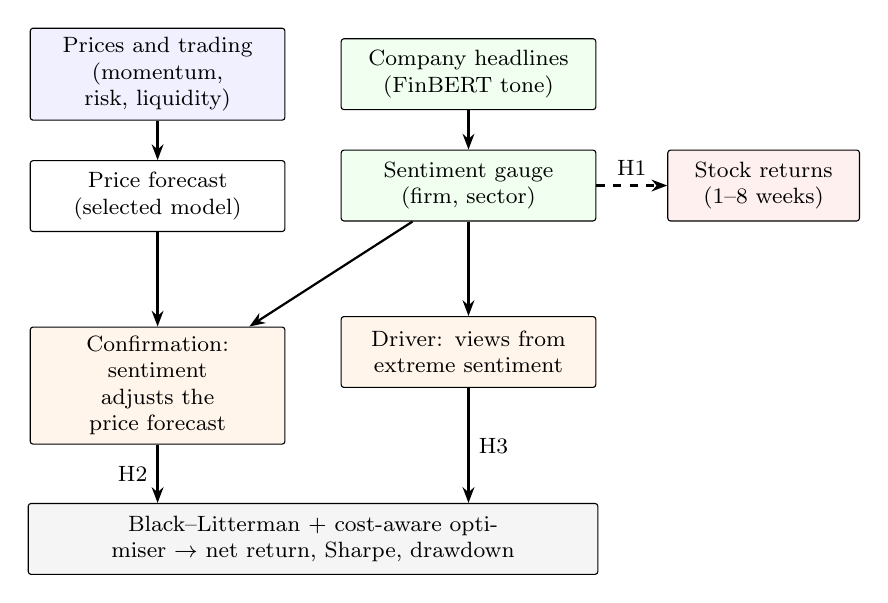
\begin{tikzpicture}[node distance=5mm and 7mm, every node/.style={font=\footnotesize, align=center},
  box/.style={draw, rounded corners=1pt, minimum height=9mm, text width=30mm, fill=#1}, box/.default=white,
  arr/.style={-{Stealth[length=2mm]}, thick}]
\node[box=blue!6] (price) {Prices and trading\\(momentum, risk, liquidity)};
\node[box=green!6, right=of price] (news) {Company headlines\\(FinBERT tone)};
\node[box, below=of price] (pf) {Price forecast\\(selected model)};
\node[box=green!6, below=of news] (sg) {Sentiment gauge\\(firm, sector)};
\node[box=orange!8, below=12mm of pf, text width=30mm] (a) {Confirmation: sentiment\\adjusts the price forecast};
\node[box=orange!8, below=12mm of sg, text width=30mm] (b) {Driver: views from\\extreme sentiment};
\node[box=gray!8, anchor=north, text width=70mm] (opt) at ($(a.south)!0.5!(b.south)+(0,-11mm)$) {Black--Litterman + cost-aware optimiser $\rightarrow$ net return, Sharpe, drawdown};
\draw[arr] (price) -- (pf); \draw[arr] (news) -- (sg); \draw[arr] (pf) -- (a); \draw[arr] (sg) -- (a); \draw[arr] (sg) -- (b);
\draw[arr] (a.south) -- node[left]{H2} (a.south |- opt.north); \draw[arr] (b.south) -- node[right]{H3} (b.south |- opt.north);
\node[box=red!6, right=9mm of sg, text width=22mm] (ret) {Stock returns\\(1--8 weeks)};
\draw[arr, dashed] (sg) -- node[above]{H1} (ret);
\end{tikzpicture}
\caption{Conceptual model. Price and news inputs form a price forecast and a sentiment gauge. Sentiment either confirms or contradicts the price-based forecast or drives the views itself. Labels show where each hypothesis is tested.}\label{fig:concept}
\end{figure}
\begin{multicols}{2}

\section{Data description}\label{sec:data}
\subsection{Sources and universe}
All data are public. The universe is the members of the S\&P~100 and the EURO STOXX~50 on 31 December 2014, the day before the test period, so membership is not chosen with hindsight. Of these 150 firms (100 and 50), nine lack a usable price history in the free data and are excluded: eight were acquired, merged or taken private between 2016 and 2025, and one has only a stale secondary listing. This leaves \Firms{} firms, \FirmsUS{} in the United States and \FirmsEU{} in the euro area, in ten sectors (Appendix~\ref{app:universe}). The exclusion uses later information; it affects 6\% of the names, and the sign of the bias is unknown because takeover targets often gain when a bid is announced. Unilever is represented by its London line, as its Amsterdam line ended with the 2020 unification.

Daily prices, volume, exchange rates and the MSCI World benchmark (the URTH fund, with dividends) come from Yahoo Finance from 2005, and the risk-free rate is the three-month U.S. Treasury yield. Returns are in U.S. dollars, unhedged. Vivendi leaves the universe at its December 2024 break-up.

Headlines come from Google News searches on each company's name, one query per firm and calendar month from October 2010 to December 2025, retrieved in October 2026. Google returns at most 100 items per query, so heavily covered firms are sampled.

\subsection{Preparation and quality}
Figure~\ref{fig:retention} shows how \Retrieved{} retrieved items become \Headlines{} company headlines. Duplicates are removed, and a headline is kept only if it names the issuer. Names that are also common words or people, such as Apple or Ford, must appear together with business words. Market roundups naming three or more firms (\Roundups{} headlines) are removed.
\end{multicols}
\begin{figure}[H]\centering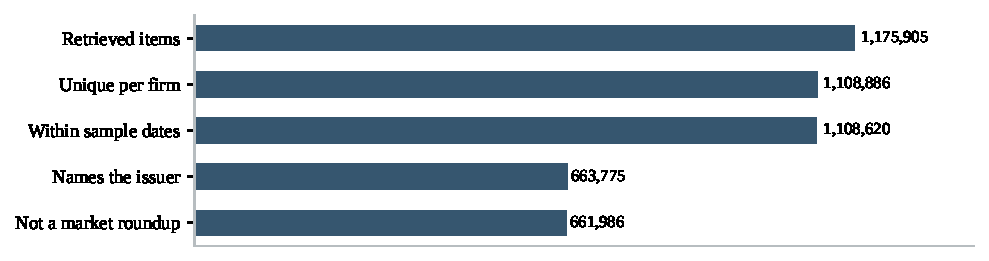
\includegraphics[width=\textwidth]{retention}
\caption{Headline retention from retrieval to the weekly decision panel.}\label{fig:retention}\end{figure}
\begin{multicols}{2}

Most headlines are close to neutral, while about \TonePositiveShare{} are clearly positive and \ToneNegativeShare{} clearly negative ($|s|>0.5$; Figure~\ref{fig:tone}). Euro-area headlines are more positive than U.S. headlines, and tone rose after 2020; such level differences are why tone is measured against each firm's own history.
\end{multicols}
\begin{figure}[H]\centering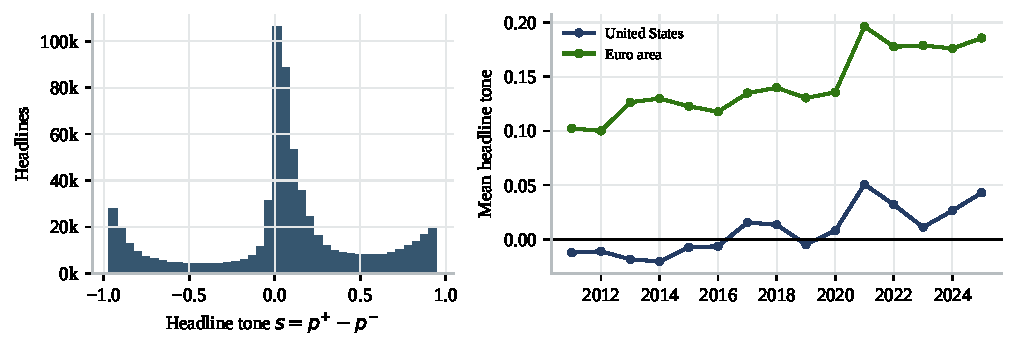
\includegraphics[width=\textwidth]{tone}
\caption{FinBERT tone of the accepted headlines: distribution (left) and annual mean by region (right).}\label{fig:tone}\end{figure}
\begin{multicols}{2}

Google News reports only the publication date, so a headline counts only from the next opening of the issuer's exchange. Coverage is uneven across firms and sectors (Figure~\ref{fig:coverage}); the median firm has \MedianHeadlinesWeek{} headlines a week, and no news arrives in \NoNewsShare{} of test stock-weeks, which then carry neutral sentiment.

\section{Methodology}\label{sec:methods}
\subsection{Research design}
The study is a quantitative simulation organised by the six phases of the Cross-Industry Standard Process for Data Mining (CRISP-DM)~\cite{chapman} (Figure~\ref{fig:design}). Decisions are weekly and walk-forward (Section~\ref{sec:model}), and all strategies share one optimiser, constraints and costs, so differences come from how sentiment enters the decision. All choices were made on the validation period, 2012--2014, then fixed with a cryptographic hash of the code and settings before the test period, January 2015 to December 2025 (\Weeks{} weeks), was run once (Figure~\ref{fig:timeline}).
\end{multicols}
\begin{figure}[H]\centering
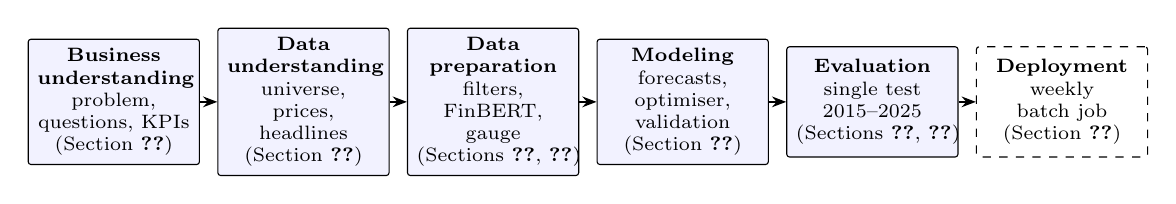
\begin{tikzpicture}[node distance=2.2mm, every node/.style={font=\scriptsize, align=center},
  phase/.style={draw, rounded corners=1pt, text width=19.4mm, minimum height=14mm, fill=blue!5,
    execute at begin node={\hyphenpenalty=10000\relax}},
  arr/.style={-{Stealth[length=1.8mm]}, thick}]
\node[phase] (b) {\textbf{Business}\\\textbf{understanding}\\problem, questions, KPIs\\(Section~\ref{sec:intro})};
\node[phase, right=of b] (d) {\textbf{Data}\\\textbf{understanding}\\universe, prices, headlines\\(Section~\ref{sec:data})};
\node[phase, right=of d] (p) {\textbf{Data}\\\textbf{preparation}\\filters, FinBERT, gauge\\(Sections~\ref{sec:prep},~\ref{sec:gauge})};
\node[phase, right=of p] (m) {\textbf{Modeling}\\forecasts, optimiser, validation\\(Section~\ref{sec:methods})};
\node[phase, right=of m] (e) {\textbf{Evaluation}\\single test 2015--2025\\(Sections~\ref{sec:results},~\ref{sec:analysis})};
\node[phase, dashed, fill=white, right=of e] (u) {\textbf{Deployment}\\weekly batch job\\(Section~\ref{sec:implications})};
\draw[arr] (b)--(d); \draw[arr] (d)--(p); \draw[arr] (p)--(m); \draw[arr] (m)--(e); \draw[arr, dashed] (e)--(u);
\end{tikzpicture}
\caption{Research design following the six CRISP-DM phases~\cite{chapman}, with the sections that cover each phase. Deployment is discussed but not carried out (dashed).}\label{fig:design}
\end{figure}
\begin{figure}[H]\centering
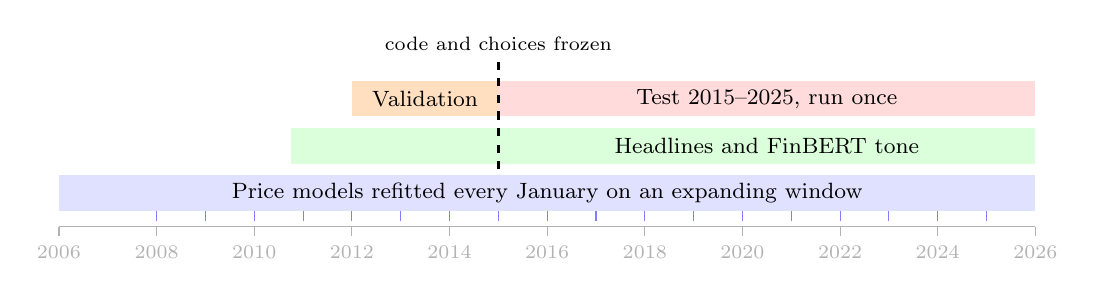
\begin{tikzpicture}[x=6.2mm, y=5mm, every node/.style={font=\footnotesize}]
\foreach \yr in {2006,2008,...,2026} {\draw[gray!60] (\yr-2005,0) -- (\yr-2005,-0.25) node[below, font=\scriptsize] {\yr};}
\draw[gray!60] (1,0) -- (21,0);
\fill[blue!12] (1,0.4) rectangle (21,1.3); \node at (11,0.85) {Price models refitted every January on an expanding window};
\fill[green!14] (5.75,1.6) rectangle (21,2.5); \node at (15.5,2.05) {Headlines and FinBERT tone};
\fill[orange!25] (7,2.8) rectangle (10,3.7); \node at (8.5,3.25) {Validation};
\fill[red!14] (10,2.8) rectangle (21,3.7); \node at (15.5,3.25) {Test 2015--2025, run once};
\draw[very thick, dashed] (10,1.45) -- (10,4.2) node[above, font=\scriptsize] {code and choices frozen};
\foreach \yr in {2008,...,2025} {\draw[blue!50] (\yr-2005,0.4) -- (\yr-2005,0.15);}
\end{tikzpicture}
\caption{Walk-forward timeline. Models are refitted every January (ticks) on data known before the first decision of the year; all choices are fixed on 2012--2014 before the test.}\label{fig:timeline}
\end{figure}
\begin{multicols}{2}

\subsection{Price forecasting models}
Six candidates represent these families: Ridge regression as the linear baseline~\cite{hoerl}, ARIMA per stock (order chosen by AIC), the factor composite, a random forest, gradient-boosted trees and an LSTM on the last eight weeks of inputs. The learning models use ten price and trading predictors (Table~\ref{tab:features}), ranked across stocks every week, and forecast returns relative to the cross-sectional mean. Fundamentals are not used because free point-in-time accounting data are unavailable for European firms. All models are pooled across stocks and refitted every January. The candidate with the highest mean weekly rank IC in the validation period is selected.
\end{multicols}
\begin{table}[H]\centering\footnotesize
\begin{tabularx}{\textwidth}{>{\raggedright\arraybackslash}p{29mm}>{\raggedright\arraybackslash}X}\toprule
Group & Inputs (values known at the decision cutoff)\\\midrule
Price (7) & 12-month momentum excluding the last month; 1-month and 1-week reversal; 60-day volatility; largest daily return over 20 days; beta to the universe over 52 weeks; distance to the 52-week high\\
Trading activity (3) & 20-day dollar volume; illiquidity (mean absolute daily return per dollar traded); abnormal volume (20-day versus 120-day dollar volume)\\
Sentiment & abnormal firm tone and abnormal sector tone (Eq.~\ref{eq:abnormal}), smoothed into the gauge\\\bottomrule
\end{tabularx}
\caption{Model inputs. Headline counts enter only through the shrinkage in Eq.~(\ref{eq:abnormal}).}\label{tab:features}
\end{table}
\begin{multicols}{2}

\subsection{Sentiment gauge}\label{sec:gauge}
The gauge combines the smoothed firm and sector scores, $G = [(1 - w)\, M^{f} + w\, M^{s}] / \mathrm{s.d.}$, where the firm-only ($w = 0$) and sector-only ($w = 1$) versions are $G^{f}$ and $G^{s}$. Validation chose between $w = 0$ and $w = 0.5$ by the larger absolute IC, and the sign of that IC decides whether the gauge is used for continuation or reversal. The s.d.\ is pooled across firms over the previous 52 weeks, which keeps the bands comparable as coverage grows. A view opens at $|G| \ge 1.5$ and closes below $|G| = 0.5$ (Figure~\ref{fig:gauge}).
\end{multicols}
\begin{figure}[H]\centering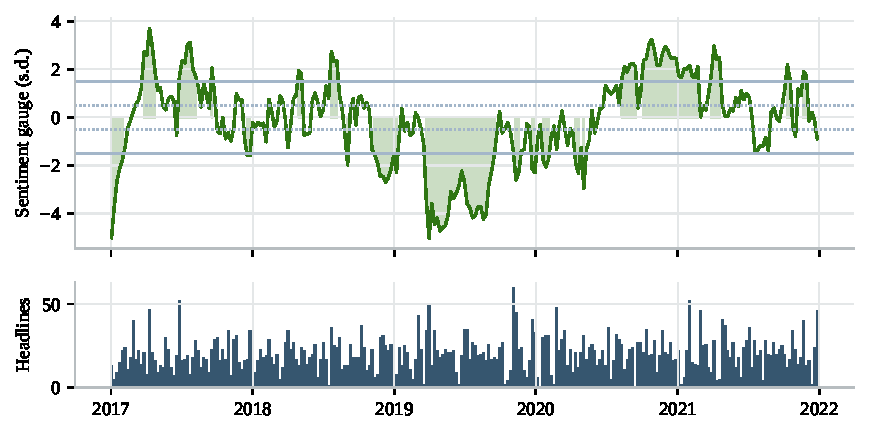
\includegraphics[width=\textwidth]{gauge_example}
\caption{Sentiment gauge and weekly headlines for Boeing, 2017--2021. Solid lines mark the entry bands and dotted lines the exit bands; shaded areas are weeks with the gauge beyond the entry band.}\label{fig:gauge}\end{figure}
\begin{multicols}{2}

\subsection{Sentiment as confirmation of the price forecast}
The selected price forecast is first converted into an expected relative return $\hat y^{P}$ by a regression through the origin of realised relative returns on the forecast over the previous three years. A Ridge model then learns how sentiment corrects the forecast. To avoid look-ahead, it is trained only on \emph{out-of-sample} errors $e = y - \hat y^{P}$, from forecasts made with earlier data, and is refitted every January:
\begin{equation}\label{eq:correction}
\begin{aligned}
\hat y^{C}_{i,t} &= \hat y^{P}_{i,t} + \beta_0 + \boldsymbol\beta^{\top} \mathbf x_{i,t} ,\\[2pt]
\mathbf x_{i,t} &= \bigl(\mathbf g_{i,t} ,\; d_{i,t}\, \mathbf g_{i,t}\bigr) ,\\[2pt]
\mathbf g_{i,t} &= \bigl(G^{f} ,\, G^{s} ,\, a^{f} ,\, a^{s}\bigr)_{i,t} ,
\end{aligned}
\end{equation}
where $G^{f}$ and $G^{s}$ are the firm and sector gauges, $a^{f}$ and $a^{s}$ the current week's abnormal firm and sector tone (Eq.~\ref{eq:abnormal}), and $d_{i,t} = \pm 1$ the direction of the price forecast; a simpler version without the weekly tone was rejected on validation. The agreement terms $d\,\mathbf g$ let sentiment strengthen a price signal it confirms and weaken, or overturn, one it contradicts. The Ridge penalty is chosen by generalised cross-validation~\cite{hoerl}.

\subsection{Optimisation model}\label{sec:model}
All optimised strategies solve the same problem every week (Table~\ref{tab:model}). The decision variables are the weights $\mathbf w$ of the $N_t$ investable stocks, which solve
\begin{equation}\label{eq:optimiser}
\begin{aligned}
\max_{\mathbf w}\;\; &\underbrace{\boldsymbol\mu^{\top} \mathbf w}_{\text{return}} \;-\; \underbrace{\frac{\delta}{2}\, \mathbf w^{\top} \boldsymbol\Sigma\, \mathbf w}_{\text{risk}} \;-\; \underbrace{\frac{c}{H} \sum_i \lvert w_i - \tilde w_i \rvert}_{\text{trading cost}}\\[4pt]
\text{s.t.}\;\; &\textstyle\sum_i w_i = 1 , \qquad 0 \le w_i \le 0.05 \quad \forall i ,
\end{aligned}
\end{equation}
a convex quadratic programme, where $\tilde{\mathbf w}$ are last week's weights after price drift. A trade is paid once but earns over several weeks, so its cost $c$ is spread over the expected holding time $H$.

The expected returns $\boldsymbol\mu$ are the Black--Litterman posterior around the reference portfolio, equal weighting. Its implied returns $\boldsymbol\pi = \delta \boldsymbol\Sigma\, \mathbf w_{\mathrm{EW}}$ make $\mathbf w_{\mathrm{EW}}$ optimal when there are no views and no costs. A view states that stock $i$ will beat $\pi_i$ by $\alpha_i = \widehat{\mathrm{IC}}_t\, \sigma_i\, z_i$, where $\sigma_i$ is its weekly volatility and $z_i$ the signal in standard deviations. With prior uncertainty $\tau\boldsymbol\Sigma$ and view uncertainty $\boldsymbol\Omega = \tau \mathbf D_S$~\cite{blacklitterman,helitterman}, $\tau$ cancels:
\begin{equation}\label{eq:bl}
\boldsymbol\mu = \boldsymbol\pi + \boldsymbol\Sigma_{\cdot S} \bigl(\boldsymbol\Sigma_{SS} + \mathbf D_S\bigr)^{-1} \boldsymbol\alpha_S ,
\end{equation}
where $S$ is the set of stocks with views, $\boldsymbol\Sigma_{\cdot S}$ the covariance of all stocks with them and $\mathbf D_S$ their variances.

The \emph{confidence} in a view enters through $\boldsymbol\Omega$, which makes each view as uncertain as the stock's own return in the prior, so a single uncorrelated view moves $\mu_i$ halfway from $\pi_i$ to $\pi_i + \alpha_i$. The size of the view follows the signal's record, as $\widehat{\mathrm{IC}}_t$ is its mean weekly rank IC over the previous three years, set to zero if negative or if fewer than 52 weeks are known, so a signal without measured skill has no views.

The strategies differ only in their views: \emph{price only} (all stocks; $z$ is the cross-sectional z-score of the price forecast), \emph{price + sentiment} (all stocks; Eq.~\ref{eq:correction}) and \emph{sentiment-driven} (only stocks with an open gauge view; $z = G$, capped at $\pm 3$). \emph{Minimum variance} solves Eq.~(\ref{eq:optimiser}) with $\boldsymbol\mu = \mathbf 0$. Benchmarks are equal weighting, rebalanced weekly, and buy-and-hold URTH. The rebalancing rule is the same every week:
\begin{enumerate}
\item At the cut-off, Thursday 22:00 UTC after the U.S. close, form the investable set (stocks with at least 40 of the last 52 weekly returns), $\boldsymbol\Sigma$, the signals and $\widehat{\mathrm{IC}}_t$ from data published before it.
\item Compute $\boldsymbol\mu$ (Eq.~\ref{eq:bl}) and solve Eq.~(\ref{eq:optimiser}) from $\tilde{\mathbf w}$.
\item Trade to the solution at each stock's Friday close, selling stocks that leave the universe, and pay $c \sum_i |w_i - \tilde w_i|$.
\item Hold for one week; the drifted weights become $\tilde{\mathbf w}$.
\end{enumerate}
\end{multicols}
\begin{table}[H]\centering\footnotesize
\begin{tabularx}{\textwidth}{>{\raggedright\arraybackslash}p{30mm}>{\raggedright\arraybackslash}X>{\raggedright\arraybackslash}p{36mm}}\toprule
Element & Specification & Setting\\\midrule
Decision variables & Weight $w_i$ of each investable stock after the weekly trade & $N_t$ = 140--141 stocks\\
Objective & Maximise expected return minus risk and trading-cost penalties, Eq.~(\ref{eq:optimiser}) & --\\
Risk term & $\frac{\delta}{2}\mathbf w^{\top}\boldsymbol\Sigma\mathbf w$; Ledoit--Wolf covariance of the last 52 weekly USD returns~\cite{ledoitwolf} & $\delta=2.5$\\
Trading-cost term & $\frac{c}{H}\sum_i|w_i-\tilde w_i|$ from the drifted weights $\tilde{\mathbf w}$ & $c=10$ bp, $H=4$ weeks\\
Reference portfolio & Equal weight; implied returns $\boldsymbol\pi=\delta\boldsymbol\Sigma\mathbf w_{\mathrm{EW}}$ & $w_i=1/N_t$\\
Expected returns & Black--Litterman posterior, Eq.~(\ref{eq:bl}) & $\tau$ cancels\\
Views & $\alpha_i=\widehat{\mathrm{IC}}_t\,\sigma_i\,z_i$ on the stocks in $S$ & gauge capped at $\pm3$\\
View confidence & $\boldsymbol\Omega=\tau\,\mathrm{diag}(\boldsymbol\Sigma_{SS})$; view size scaled by the trailing IC & 3-year IC, $\ge$52 weeks, floored at 0\\
Constraints & Fully invested, long-only, issuer limit (UCITS 5\%); no leverage, cash or sector limits & $\sum_i w_i=1$, $0\le w_i\le0.05$\\
Rebalancing & Decide Thursday 22:00 UTC, trade at each stock's Friday close, hold one week & \Weeks{} weekly decisions\\
Solver & Convex quadratic programme & Clarabel (cvxpy)\\\bottomrule
\end{tabularx}
\caption{Specification of the optimisation model shared by all optimised strategies; minimum variance sets $\boldsymbol\mu=\mathbf 0$.}\label{tab:model}
\end{table}
\begin{multicols}{2}

\subsection{Costs and evaluation}
Every purchase and sale costs $c = 10$ basis points of traded value, close to the measured costs of large institutional trades~\cite{frazzini}; 0, 5 and 20 basis points are tested. KPIs are compound annual growth (CAGR), volatility, the Sharpe and Sortino ratios (Treasury yield as risk-free rate), maximum drawdown, turnover and cost. Differences between strategies get 95\% intervals from a paired bootstrap that resamples 13-week blocks to keep autocorrelation (2,000 draws)~\cite{politis}; mean ICs and alphas use Newey--West (HAC) standard errors~\cite{neweywest}. RQ1 is tested with an event study of daily returns relative to the stock's regional average around tradable gauge signals, and with Fama--MacBeth regressions of next-week returns on the gauges with and without price controls~\cite{famamacbeth}. Robustness tests change one setting at a time. Table~\ref{tab:decisions}, Figure~\ref{fig:mechanism}, Section~\ref{sec:coverage} and Appendix~\ref{app:fnspid} report analyses added after the test; they use the frozen models and change no choice.

\section{Results}\label{sec:results}
\subsection{Model selection on the validation period}
No price model forecast weekly returns reliably in 2012--2014 (Table~\ref{tab:selection}). The factor composite had the highest mean rank IC, \ValFactorIC{} ($t=\ValFactorT$), and was selected. The firm + sector gauge had a higher IC than the firm-only gauge (\ValGaugeFirmSectorIC{} against \ValGaugeFirmIC{}) and a positive sign, so it was used for continuation. Adding the weekly abnormal tone to the sentiment correction raised its validation IC from +0.0090 to +0.0108 (gain $t=0.06$), so that version was kept.
\end{multicols}
\begin{table}[H]\centering\footnotesize\begin{tabular}{lrrr}
\toprule
Model & Mean rank IC & HAC $t$ & Weeks IC $>0$ (\%) \\
\midrule
Ridge regression & -0.0040 & -0.25 & 49.7 \\
\textbf{Factor composite} & +0.0090 & 0.39 & 54.1 \\
ARIMA & -0.0038 & -0.39 & 47.1 \\
Random forest & -0.0000 & -0.00 & 52.2 \\
Gradient boosting & +0.0018 & 0.20 & 49.7 \\
LSTM & -0.0031 & -0.13 & 47.1 \\
\midrule
Sentiment gauge, firm only & +0.0039 & 0.60 & 51.6 \\
\textbf{Sentiment gauge, firm + sector} & +0.0125 & 0.98 & 55.4 \\
\bottomrule
\end{tabular}

\caption{Validation results, 2012--2014 (157 weeks). Rank IC with Newey--West (HAC) $t$-statistics; selected models in bold.}\label{tab:selection}\end{table}
\begin{multicols}{2}

\subsection{Sentiment and future returns (RQ1)}
Figure~\ref{fig:event} follows \EventPosN{} positive and \EventNegN{} negative gauge signals. Most of the abnormal return comes \emph{before} the signal can be traded, with \EventPosPre{} and \EventNegPre{} in the ten days up to day~0. After day~0, positive signals drift up by a further \EventPosPost{} over 20 trading days and then fall back (\EventPosPostForty{} from day~0 to day~40), while negative signals move by \EventNegPost{} over 20 days and then recover (\EventNegPostForty{}). Over 20 days both groups move in the expected direction, but by amounts small relative to the intervals that fade by day~40, so H1a is supported in direction only.
\end{multicols}
\begin{figure}[H]\centering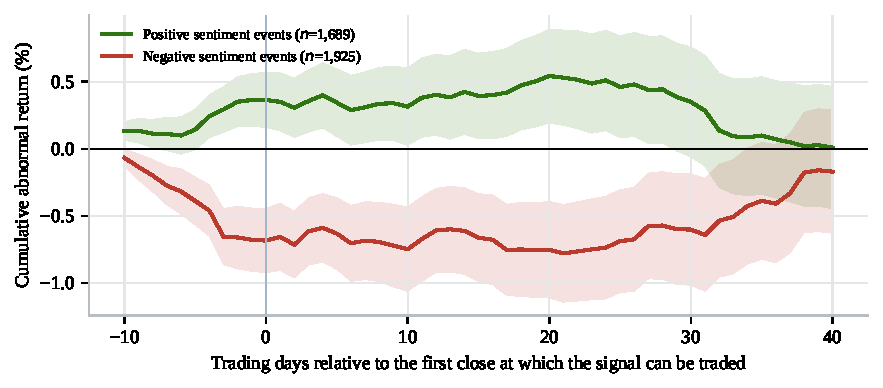
\includegraphics[width=\textwidth]{event_study}
\caption{Cumulative abnormal return (relative to the equal-weighted return of the stock's region) around gauge signals, 2015--2025, with 95\% intervals. Day~0 is the first close at which the signal can be traded.}\label{fig:event}\end{figure}
\begin{multicols}{2}

In Fama--MacBeth regressions (Table~\ref{tab:fm}), a one-standard-deviation higher firm gauge predicts a \FMCtrlFirm{} basis points higher relative return the next week after price controls ($t=\FMCtrlFirmT$), \FMUSFirm{} basis points in the United States ($t=\FMUSFirmT$) and \FMEUFirm{} in the euro area ($t=\FMEUFirmT$). Sector sentiment is insignificant. H1b is supported in direction only for firm sentiment. Over horizons of one to eight weeks the gauge's rank IC is near zero, with its highest value, \DecaySentimentFour{} ($t=\DecaySentimentFourT$), four weeks ahead (Figure~\ref{fig:decay}).
\end{multicols}
\begin{figure}[H]\centering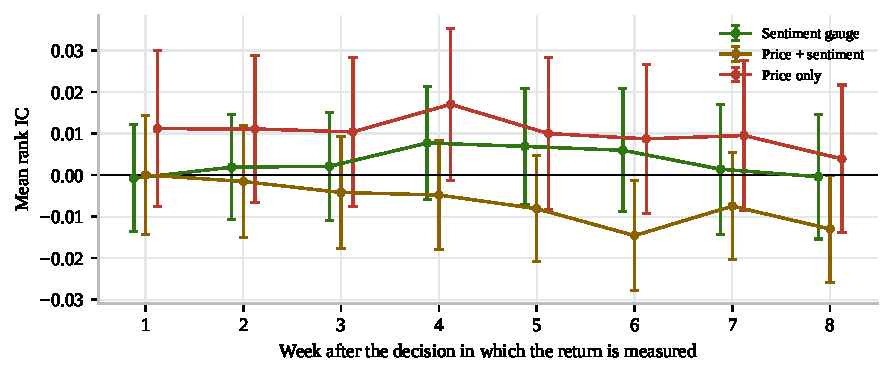
\includegraphics[width=0.85\textwidth]{decay}
\caption{Mean rank IC of each signal for returns one to eight weeks after the decision, with 95\% intervals.}\label{fig:decay}\end{figure}
\begin{table}[H]\centering\footnotesize\begin{tabular}{lcccc}
\toprule
Regressor & Sentiment only & With price controls & U.S. & Euro area \\
\midrule
Firm sentiment gauge & +1.1 (0.97) & +1.3 (1.19) & +2.2 (1.61) & -0.9 (-0.45) \\
Sector sentiment gauge & -1.9 (-0.79) & -0.8 (-0.41) & -1.1 (-0.51) & -0.9 (-0.37) \\
Momentum 12-1 &  & +1.5 (0.55) & +2.5 (0.83) & +2.3 (0.72) \\
Reversal (1 month) &  & +4.9 (1.59) & +5.6 (1.47) & +3.5 (1.24) \\
Volatility (60 days) &  & -3.4 (-0.99) & -2.5 (-0.69) & -2.4 (-0.67) \\
Dollar volume &  & +3.3 (1.22) & +3.5 (1.63) & -3.9 (-1.94) \\
Beta (52 weeks) &  & +7.5 (1.49) & +4.7 (0.87) & +7.2 (1.58) \\
Mean $R^2$ & 0.036 & 0.242 & 0.271 & 0.326 \\
\bottomrule
\end{tabular}

\caption{Fama--MacBeth regressions of next-week relative returns on standardised predictors, 2015--2025. Coefficients in basis points per standard deviation, Newey--West $t$-statistics in parentheses.}\label{tab:fm}\end{table}
\begin{multicols}{2}

\subsection{Sentiment as confirmation of the price forecast (RQ2)}
In the test period the factor composite kept a small positive IC, \ICPrice{} ($t=\ICPriceT$), while the corrected forecast fell to \ICCombined{} ($t=\ICCombinedT$) and the gauge itself had an IC of \ICSentiment{} ($t=\ICSentimentT$). Table~\ref{tab:decisions} shows the hit rates behind this result. The price signal and the sentiment gauge were each right about half of the time, whether they agreed or disagreed. When the correction moved a stock to the other side of the average (\DecChangedShare{} of cases), the original price decision would have been right more often than the new one (\DecChangedPrice{} against \DecChangedComb{}).
\end{multicols}
\begin{table}[H]\centering\footnotesize
\begin{tabular}{lccc}\toprule
\multicolumn{4}{l}{\emph{A. Did each signal pick the right side of the average?}}\\
Situation & Share of cases & Price signal right & Sentiment right\\\midrule
Price and sentiment agree & \DecAgreeShare & \DecAgreePrice & \DecAgreeSent\\
Price and sentiment disagree & \DecDisagreeShare & \DecDisagreePrice & \DecDisagreeSent\\
Sentiment neutral & \DecNeutralShare & \DecNeutralPrice & \DecNeutralSent\\
All cases & \DecAllShare & \DecAllPrice & \DecAllSent\\\midrule
\multicolumn{4}{l}{\emph{B. Decisions changed by the sentiment correction}}\\
 & Share of cases & Original price decision right & Corrected decision right\\\midrule
Correction moved the stock to the other side & \DecChangedShare & \DecChangedPrice & \DecChangedComb\\\bottomrule
\end{tabular}
\caption{Who was right? One case is one stock in one week, 2015--2025. A signal is right when the stock it favours (penalises) does better (worse) than the average stock the next week; a coin flip is right 50\% of the time. Sentiment agrees or disagrees when its gauge is at least 0.5 s.d. on the same or the opposite side of the price signal; cases with a gauge of exactly zero are left out of ``Sentiment right''.}\label{tab:decisions}\end{table}
\begin{multicols}{2}

The portfolio results are better than the forecast results (Table~\ref{tab:performance}). The price + sentiment portfolio earned \CombinedCAGR{} a year with a Sharpe ratio of \CombinedSharpe{} and a maximum drawdown of \CombinedDD{}, against \PriceCAGR{}, \PriceSharpe{} and \PriceDD{} for price only; the difference, \BootCombinedPriceCAGR{} percentage points a year, has a 95\% interval of [\BootCombinedPriceCAGRLow, \BootCombinedPriceCAGRHigh] (Table~\ref{tab:uncertainty}). Figure~\ref{fig:mechanism} shows where the difference arises. As a simple average, the gain of \NetCombinedPrice{} percentage points a year splits into \GrossCombinedPrice{} before costs and \SavingCombinedPrice{} from lower costs. The before-cost gain came equally from the price portfolio's buy decisions (stocks it overweighted; \SideBuyGain{} percentage points a year, $t=\SideBuyGainT$) and sell decisions (stocks it underweighted; \SideSellGain, $t=\SideSellGainT$). When sentiment enlarged a buy or a sell, the stock moved the intended way in \SideBuyLargerRight{} and \SideSellLargerRight{} of cases. H2a and H2b are supported in direction but not statistically, and H2c in direction only: stocks moved \DecAgreeRet{} basis points a week in the price signal's direction when sentiment agreed and \DecDisagreeRet{} when it disagreed (both insignificant).
\end{multicols}
\begin{figure}[H]\centering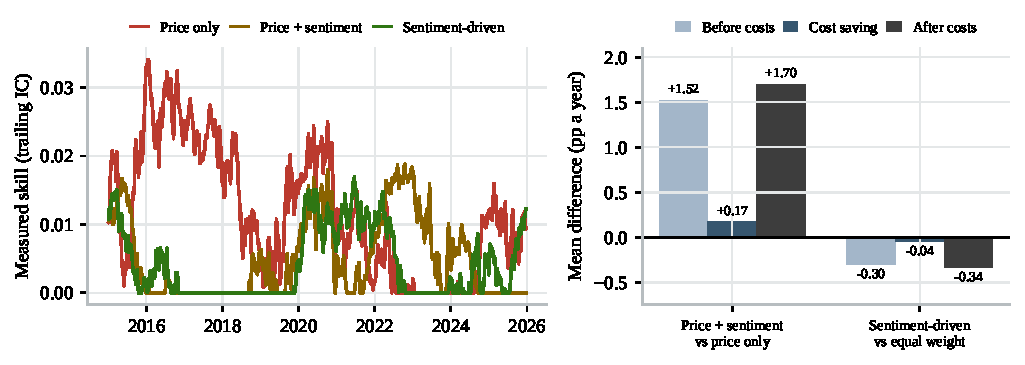
\includegraphics[width=\textwidth]{allocation_mechanism}
\caption{Left: measured skill (trailing three-year rank IC, floored at zero) that scales each signal's views. Right: mean annual return difference before costs, from lower costs and after costs (arithmetic, percentage points).}\label{fig:mechanism}\end{figure}
\begin{multicols}{2}

\subsection{Sentiment as the driver of the allocation (RQ3)}
Driven by sentiment alone, the portfolio held about \SentimentHoldings{} stocks with views on \SentimentViews{} of them in an average week; in \ZeroSkillSentiment{} of the weeks the gauge's trailing IC was zero and the optimiser moved towards equal weighting. The portfolio earned \SentimentCAGR{} a year, slightly less than equal weighting (\EWCAGR), but with a Sharpe ratio of \SentimentSharpe{}, against \EWSharpe{} for equal weighting, \MinVarSharpe{} for minimum variance and \IndexSharpe{} for MSCI World (Figure~\ref{fig:wealth}; drawdowns and annual returns in Appendix~\ref{app:annual}). Its maximum drawdown, \SentimentDD{}, was smaller than that of equal weighting (\EWDD{}) and the index (\IndexDD{}). All differences have bootstrap intervals that include zero (Table~\ref{tab:uncertainty}). H3 is supported in direction only.
\end{multicols}
\begin{table}[H]\centering\footnotesize\setlength{\tabcolsep}{4pt}\begin{tabular}{lrrrrrrrrr}
\toprule
Strategy & CAGR & Vol. & Sharpe & Sortino & Max DD & Turnover & Costs & $\alpha$ ($t$) & $\beta$ \\
\midrule
Sentiment-driven & 11.90 & 16.77 & 0.64 & 0.89 & -31.6 & 1.6 & 0.17 & +1.59 (+0.67) & 0.91 \\
Price + sentiment & 12.20 & 16.86 & 0.65 & 0.93 & -30.4 & 3.5 & 0.36 & +1.62 (+0.81) & 0.93 \\
Price only & 10.28 & 16.99 & 0.54 & 0.76 & -34.4 & 5.2 & 0.54 & -0.11 (-0.05) & 0.94 \\
Minimum variance & 9.41 & 13.05 & 0.60 & 0.81 & -28.2 & 0.5 & 0.05 & +1.15 (+0.55) & 0.67 \\
Equal weight & 12.15 & 17.46 & 0.63 & 0.90 & -36.7 & 1.2 & 0.13 & +1.30 (+0.65) & 0.97 \\
MSCI World (URTH) & 11.18 & 16.59 & 0.60 & 0.85 & -32.7 & -- & -- & -- & -- \\
\bottomrule
\end{tabular}

\caption{Net performance, January 2015 to December 2025 (\Weeks{} weeks), 10 bp per trade. CAGR, volatility, costs and alpha in \% a year; turnover is the average weekly one-way turnover in \%; alpha and beta against MSCI World with Newey--West $t$-statistics.}\label{tab:performance}\end{table}
\begin{table}[H]\centering\footnotesize\setlength{\tabcolsep}{4pt}\begin{tabular}{lcccc}
\toprule
Comparison (A vs B) & Return (pp a year) & Sharpe ratio & Drawdown (pp) & Significant? \\
\midrule
Price + sentiment vs price only & +1.92 (-1.47 to +5.00) & +0.10 (-0.09 to +0.28) & +4.0 (-5.5 to +9.5) & No \\
Sentiment-driven vs equal weight & -0.25 (-3.23 to +2.72) & +0.01 (-0.15 to +0.14) & +5.1 (-3.9 to +9.1) & No \\
Sentiment-driven vs minimum variance & +2.49 (-3.09 to +8.62) & +0.03 (-0.32 to +0.34) & -3.3 (-13.9 to +2.7) & No \\
Sentiment-driven vs MSCI World & +0.72 (-4.01 to +5.76) & +0.03 (-0.24 to +0.29) & +1.1 (-6.2 to +10.4) & No \\
Price + sentiment vs equal weight & +0.06 (-2.41 to +2.56) & +0.02 (-0.12 to +0.14) & +6.3 (-4.0 to +10.7) & No \\
Price only vs equal weight & -1.86 (-5.20 to +1.43) & -0.09 (-0.26 to +0.08) & +2.2 (-5.0 to +6.8) & No \\
\bottomrule
\end{tabular}

\caption{Are the differences real? Each cell shows strategy A minus strategy B (for drawdown, how much smaller A's drawdown was) with its 95\% confidence interval in brackets (paired block bootstrap, 13-week blocks, 2,000 draws). A difference is significant only if its interval excludes zero.}\label{tab:uncertainty}\end{table}
\begin{figure}[H]\centering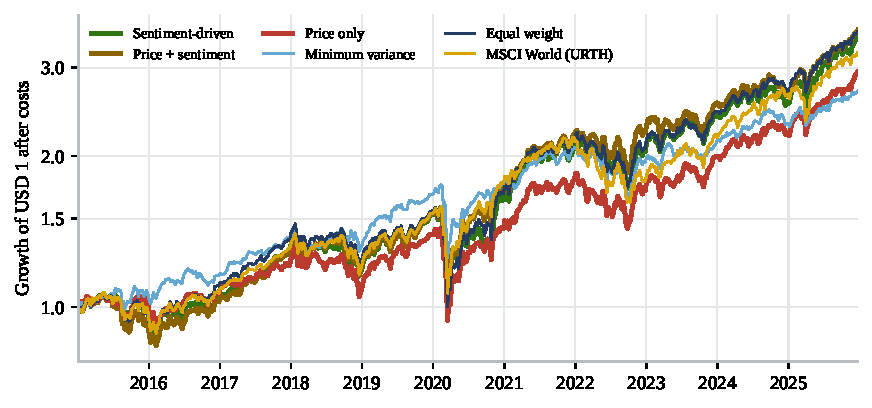
\includegraphics[width=\textwidth]{wealth}
\caption{Growth of USD~1 after costs, 2015--2025 (log scale).}\label{fig:wealth}\end{figure}
\begin{multicols}{2}

\section{Analysis}\label{sec:analysis}
\subsection{Sensitivity to costs, constraints and timing}
In Table~\ref{tab:robustness}, the sentiment-driven portfolio's Sharpe ratio stays above equal weighting with a lower entry band of 1~s.d. (\RobEntryBandOneSDSentimentSharpe), with a one- or four-week half-life, and when news reaches the portfolio one session later (\RobNewsOneSessionLaterSentimentSharpe). The higher 2~s.d. band and the 10\% position limit leave it slightly below.

The cost results are not monotonic (Figure~\ref{fig:costs}). The sentiment-driven portfolio has a higher Sharpe ratio than equal weighting at every cost level, and without costs it earns \RobCostsZeroBpPerTradeSentimentCAGR{} a year against \RobCostsZeroBpPerTradeEWCAGR{}. At 20 bp all optimisers trade less, and the price-only portfolio performs best of all. A different cost rate changes the trades the optimiser makes as well as the net return, and the spread across scenarios is as large as the differences between strategies.
\end{multicols}
\begin{table}[H]\centering\footnotesize\setlength{\tabcolsep}{4pt}\begin{tabular}{lccccc}
\toprule
Scenario & Sentiment-driven & Price + sentiment & Price only & Minimum variance & Equal weight \\
\midrule
Base case & 11.90 / 0.64 & 12.20 / 0.65 & 10.28 / 0.54 & 9.41 / 0.60 & 12.15 / 0.63 \\
Costs 20 bp per trade & 12.99 / 0.70 & 12.72 / 0.70 & 13.74 / 0.75 & 10.41 / 0.66 & 12.00 / 0.62 \\
Position limit 10\% & 11.73 / 0.62 & 12.05 / 0.64 & 10.67 / 0.56 & 8.80 / 0.56 & 12.15 / 0.63 \\
Entry band 1 s.d. & 12.57 / 0.67 & -- & -- & -- & -- \\
Entry band 2 s.d. & 11.48 / 0.61 & -- & -- & -- & -- \\
Gauge half-life 1 week & 12.70 / 0.68 & 12.30 / 0.65 & -- & -- & -- \\
Gauge half-life 4 weeks & 12.13 / 0.65 & 13.02 / 0.70 & -- & -- & -- \\
News one session later & 12.29 / 0.66 & 12.40 / 0.65 & -- & -- & -- \\
2015-2019 & 8.79 / 0.62 & 8.94 / 0.62 & 6.84 / 0.50 & 10.87 / 0.93 & 9.20 / 0.65 \\
2020-2025 & 14.57 / 0.66 & 15.01 / 0.68 & 13.25 / 0.59 & 8.21 / 0.42 & 14.67 / 0.64 \\
\bottomrule
\end{tabular}

\caption{Robustness: CAGR (\%) / Sharpe ratio after costs. One setting is changed at a time; ``--'' means the strategy is unaffected. Costs of 0 and 5 bp are shown in Figure~\ref{fig:costs}.}\label{tab:robustness}\end{table}
\begin{figure}[H]\centering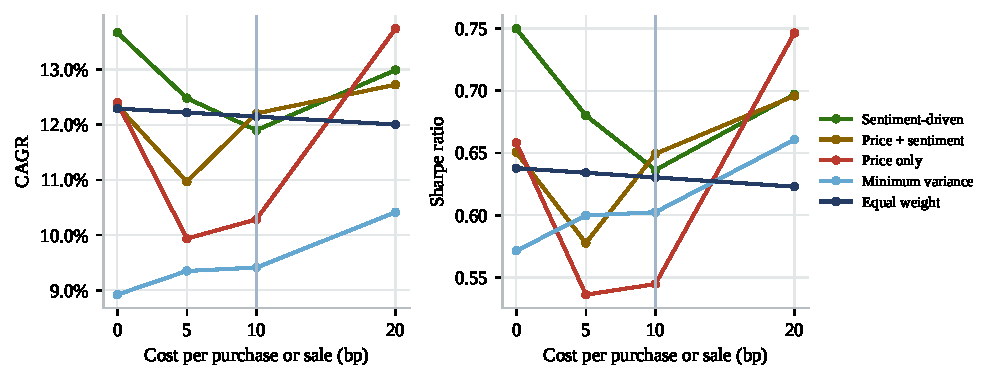
\includegraphics[width=\textwidth]{costs}
\caption{Net CAGR and Sharpe ratio as functions of the cost per purchase or sale. The vertical line marks the base case.}\label{fig:costs}\end{figure}
\begin{multicols}{2}

\subsection{Market conditions and sources of return}
In 2015--2019 minimum variance had the highest Sharpe ratio (\RobTwoZeroOneFiveTwoZeroOneNineMinVarSharpe) and the sentiment-driven portfolio trailed equal weighting slightly; in 2020--2025 the sentiment-driven and price + sentiment portfolios had the highest Sharpe ratios (\RobTwoZeroTwoZeroTwoZeroTwoFiveSentimentSharpe{} and \RobTwoZeroTwoZeroTwoZeroTwoFiveCombinedSharpe). Relative to equal weighting, the sentiment-driven portfolio returned \UpSentimentEW{} basis points a week in rising markets and \DownSentimentEW{} in falling markets (both insignificant), which suggests that its smaller drawdown comes from defensive behaviour in sell-offs.

On average the sentiment-driven portfolio held about 8 percentage points more information technology and 7 points less financials than equal weighting (Figure~\ref{fig:tilts}). Technology outperformed during the test period, so part of the result may come from this sector tilt rather than from picking stocks within sectors.
\end{multicols}
\begin{figure}[H]\centering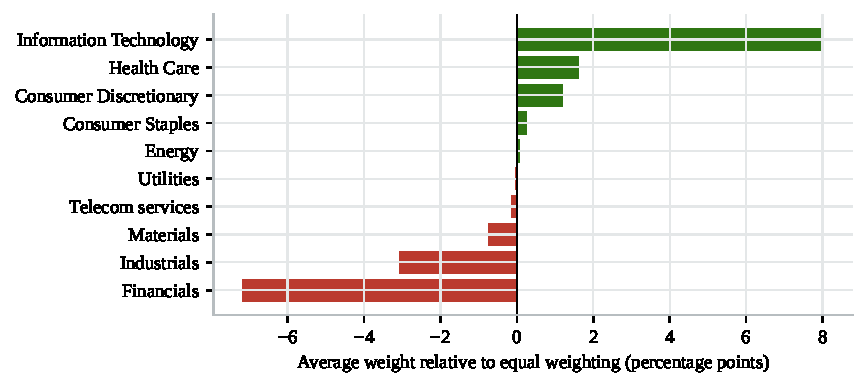
\includegraphics[width=0.8\textwidth]{sector_tilts}
\caption{Average sector weight of the sentiment-driven portfolio relative to equal weighting, 2015--2025.}\label{fig:tilts}\end{figure}
\begin{multicols}{2}

\section{Discussion}\label{sec:discussion}
\subsection{Interpretation and comparison with earlier studies}
\textbf{RQ1.} Headline sentiment in large caps mostly confirms price moves that have already happened, which fits Tetlock's temporary price pressure~\cite{tetlock2007} and the over-reaction to heavily covered news reported by Hillert et al.~\cite{hillert} better than the slow absorption of weekly tone found by Heston and Sinha~\cite{hestonsinha}. The difference is consistent with Ke et al.~\cite{kekellyxiu}, who find that news about large firms is priced within days: the firms here are heavily covered, and dates-only news reaches the portfolio a day or more after professional feeds.

\textbf{RQ2.} Like Coriat and Benhamou~\cite{coriat}, the allocation that combined price and sentiment did better than the price-only allocation, with a higher return and Sharpe ratio and a smaller drawdown. Unlike in their study, the correction did not make the forecast more accurate, and the gain is not statistically significant. The gain is still economically relevant. In liquid large caps a credible edge is expected to be small and spread over many decisions~\cite{grinoldkahn}, and an extra 1--2 percentage points a year, earned on both buy and sell decisions, matters to an investor, even if eleven years are too short to separate it from luck.

\textbf{RQ3.} Using sentiment as Black--Litterman views, as Colasanto et al.\ did~\cite{colasanto}, gave a marginally higher Sharpe ratio and a smaller drawdown than the benchmarks, with little trading. DeMiguel et al.'s warning that $1/N$ is hard to beat~\cite{demiguel} still holds: no difference is statistically significant over eleven years. In economic terms, a drawdown about five percentage points smaller than equal weighting at a similar return is valuable to an investor who must hold through sell-offs.

\subsection{Implications for portfolio managers}
The results give two guidelines. First, public headline sentiment is better used together with a price-based forecast than as a stand-alone source of alpha in liquid large caps; here it improved the allocation without improving forecast accuracy, and gains of this size justify further testing even though one sample cannot confirm them. Second, any signal should enter through a skill-weighted, cost-aware optimiser, which limits the damage when a signal stops working. Deployment is a weekly batch job of headline retrieval, FinBERT scoring and one quadratic programme, which runs in minutes on a laptop.

\subsection{Limitations and future work}
The universe excludes nine firms that later disappeared, a bias of unknown sign. The news archive was retrieved in 2026 and ranked by today's relevance, which may favour items still online and stories that later proved important. Many comparisons were made, eleven years give little power to detect Sharpe differences of about 0.1, the cost penalty was not tuned, and MSCI World also contains markets outside the universe. Weekly decisions cannot capture effects that last only hours. Future work should use a real-time news feed with time stamps, a broader mid-cap universe where news is absorbed more slowly, and a cost penalty and holding horizon chosen on the validation period.

\section{Conclusion}\label{sec:conclusion}
This study asked how news sentiment can improve the optimised allocation of a weekly, long-only U.S. and euro-area equity portfolio after costs, with all models chosen on 2012--2014 and tested once on 2015--2025.

\textbf{RQ1.} Sentiment signals mostly followed price moves; the small continuation over the next month faded by day 40 (H1a in direction only). Firm sentiment had a small, insignificant positive effect after price controls (H1b in direction only).

\textbf{RQ2.} Correcting the factor forecast with sentiment did not raise its IC, but the portfolio earned \BootCombinedPriceCAGR{} percentage points more a year with a smaller drawdown, a gain earned on both buy and sell decisions (H2a--H2c in direction only).

\textbf{RQ3.} The sentiment-driven allocation earned \SentimentCAGR{} a year, slightly below equal weighting, with a Sharpe ratio of \SentimentSharpe{}, marginally above equal weighting (\EWSharpe), minimum variance (\MinVarSharpe) and MSCI World (\IndexSharpe), and a smaller drawdown than equal weighting and the index. The differences are not significant and depend on costs and period (H3 in direction only).

Sentiment improved the allocation in direction without improving the return forecasts, and no improvement was statistically significant. Gains of one to two percentage points a year are small, but in liquid large caps they are economically relevant. For a portfolio manager, public headline sentiment is useful as a confirmation layer for a price-based allocation and weak as a source of alpha on its own.


\bibliographystyle{elsarticle-num}
\bibliography{references}
\end{multicols}

\clearpage
\appendix
\section{Universe and news coverage}\label{app:universe}
Table~\ref{tab:universe} lists the firms with their accepted headlines for October 2010--December 2025; Figure~\ref{fig:coverage} shows the average number of headlines per firm and week by sector and year.
\begin{table}[p]\centering\tiny\setlength{\tabcolsep}{3pt}\renewcommand{\arraystretch}{0.92}\begin{tabular}{llrllr}
\toprule
Ticker & Company & Headlines & Ticker & Company & Headlines \\
\midrule
BMW.DE & BMW & 16,585 & COP & ConocoPhillips & 957 \\
ITX.MC & Inditex & 856 & CVX & Chevron & 3,815 \\
MBG.DE & Daimler (Mercedes-Benz Group) & 4,070 & DVN & Devon Energy & 260 \\
MC.PA & LVMH & 4,321 & HAL & Halliburton & 1,255 \\
VIV.PA & Vivendi & 468 & NOV & National Oilwell Varco & 89 \\
VOW3.DE & Volkswagen & 16,019 & OXY & Occidental Petroleum & 1,291 \\
ABI.BR & Anheuser-Busch InBev & 3,395 & SLB & Schlumberger & 1,936 \\
BN.PA & Danone & 2,057 & XOM & Exxon Mobil & 3,949 \\
CA.PA & Carrefour & 2,226 & AIG & American International Group & 3,362 \\
OR.PA & L'Oreal & 6,314 & ALL & Allstate & 1,912 \\
ULVR.L & Unilever & 6,547 & AXP & American Express & 6,054 \\
ENI.MI & Eni & 2,009 & BAC & Bank of America & 7,448 \\
REP.MC & Repsol & 1,394 & BK & Bank of New York Mellon & 1,475 \\
TTE.PA & Total (TotalEnergies) & 4,271 & BRK-B & Berkshire Hathaway & 3,304 \\
ALV.DE & Allianz & 2,134 & C & Citigroup & 6,899 \\
BBVA.MC & BBVA & 2,110 & COF & Capital One & 4,181 \\
BNP.PA & BNP Paribas & 2,844 & GS & Goldman Sachs & 9,534 \\
CS.PA & AXA & 2,032 & JPM & JPMorgan Chase & 8,863 \\
DBK.DE & Deutsche Bank & 4,626 & MET & MetLife & 3,251 \\
G.MI & Generali & 803 & MS & Morgan Stanley & 5,510 \\
GLE.PA & Societe Generale & 1,114 & SPG & Simon Property Group & 252 \\
INGA.AS & ING Groep & 390 & USB & U.S. Bancorp & 3,685 \\
ISP.MI & Intesa Sanpaolo & 455 & WFC & Wells Fargo & 7,817 \\
MUV2.DE & Munich Re & 815 & ABBV & AbbVie & 2,015 \\
SAN.MC & Banco Santander & 2,607 & ABT & Abbott Laboratories & 2,653 \\
UCG.MI & UniCredit & 935 & AMGN & Amgen & 1,964 \\
BAYN.DE & Bayer & 2,756 & BAX & Baxter International & 1,692 \\
EL.PA & Essilor (EssilorLuxottica) & 284 & BIIB & Biogen & 1,378 \\
SAN.PA & Sanofi & 3,112 & BMY & Bristol-Myers Squibb & 1,219 \\
AIR.PA & Airbus & 11,915 & GILD & Gilead Sciences & 2,642 \\
DG.PA & Vinci & 757 & JNJ & Johnson \& Johnson & 6,174 \\
DHL.DE & Deutsche Post DHL & 5,565 & LLY & Eli Lilly & 4,391 \\
PHIA.AS & Philips & 2,641 & MDT & Medtronic & 3,135 \\
SGO.PA & Saint-Gobain & 775 & MRK & Merck \& Co. & 3,991 \\
SIE.DE & Siemens & 8,343 & PFE & Pfizer & 6,621 \\
SU.PA & Schneider Electric & 2,080 & UNH & UnitedHealth Group & 1,720 \\
ASML.AS & ASML & 1,640 & BA & Boeing & 15,084 \\
NOKIA.HE & Nokia & 10,317 & CAT & Caterpillar & 2,539 \\
SAP.DE & SAP & 3,384 & EMR & Emerson Electric & 245 \\
AI.PA & Air Liquide & 584 & FDX & FedEx & 9,757 \\
BAS.DE & BASF & 2,041 & GD & General Dynamics & 1,542 \\
DTE.DE & Deutsche Telekom & 624 & GE & General Electric & 6,682 \\
ORA.PA & Orange & 70 & HON & Honeywell & 4,170 \\
TEF.MC & Telefonica & 1,130 & LMT & Lockheed Martin & 8,471 \\
ENEL.MI & Enel & 794 & MMM & 3M & 2,017 \\
ENGI.PA & GDF Suez (Engie) & 999 & NSC & Norfolk Southern & 1,595 \\
EOAN.DE & E.ON & 575 & RTX & United Technologies (RTX) & 468 \\
IBE.MC & Iberdrola & 943 & UNP & Union Pacific & 2,180 \\
RWE.DE & RWE & 1,099 & UPS & United Parcel Service & 3,417 \\
AMZN & Amazon.com & 7,347 & AAPL & Apple & 15,758 \\
CMCSA & Comcast & 6,589 & ACN & Accenture & 5,115 \\
DIS & Walt Disney & 15,723 & CSCO & Cisco Systems & 7,165 \\
F & Ford Motor & 6,189 & EBAY & eBay & 12,534 \\
GM & General Motors & 8,799 & GOOGL & Google (Alphabet) & 13,809 \\
HD & Home Depot & 6,777 & HPQ & Hewlett-Packard (HP Inc) & 1,182 \\
LOW & Lowe's & 3,021 & IBM & IBM & 9,164 \\
MCD & McDonald's & 15,468 & INTC & Intel & 14,687 \\
NKE & Nike & 6,195 & MA & Mastercard & 6,149 \\
SBUX & Starbucks & 14,342 & META & Facebook (Meta Platforms) & 16,273 \\
TGT & Target & 6,184 & MSFT & Microsoft & 12,010 \\
CL & Colgate-Palmolive & 818 & ORCL & Oracle & 5,346 \\
COST & Costco & 10,795 & QCOM & Qualcomm & 6,955 \\
CVS & CVS Health & 7,747 & TXN & Texas Instruments & 800 \\
KO & Coca-Cola & 13,440 & V & Visa & 1,794 \\
MDLZ & Mondelez International & 2,436 & DD & DuPont & 4,819 \\
MO & Altria & 716 & FCX & Freeport-McMoRan & 436 \\
PEP & PepsiCo & 11,284 & T & AT\&T & 11,195 \\
PG & Procter \& Gamble & 4,939 & VZ & Verizon & 10,460 \\
PM & Philip Morris International & 1,825 & EXC & Exelon & 437 \\
WMT & Walmart & 16,087 & SO & Southern Company & 404 \\
APA & Apache & 87 &  &  &  \\
\bottomrule
\end{tabular}

\caption{Research universe: members of the S\&P~100 and EURO STOXX~50 on 31 December 2014 with usable price histories, and their accepted headlines.}\label{tab:universe}\end{table}
\begin{figure}[H]\centering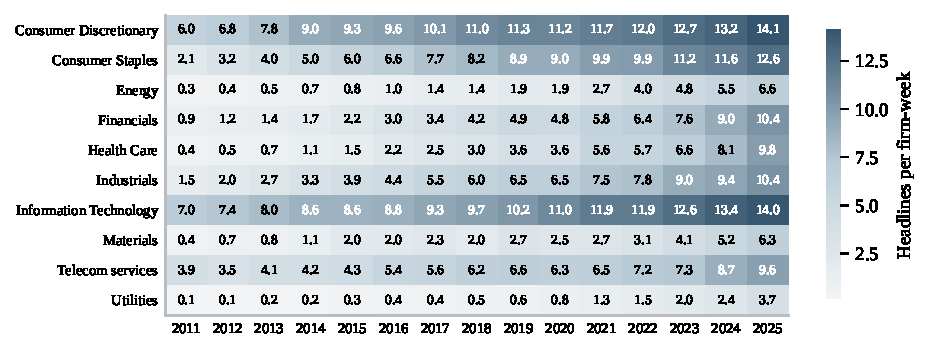
\includegraphics[width=\textwidth]{coverage}
\caption{Accepted headlines per firm and week, by sector and year.}\label{fig:coverage}\end{figure}

\section{Drawdowns and annual returns}\label{app:annual}
\begin{figure}[H]\centering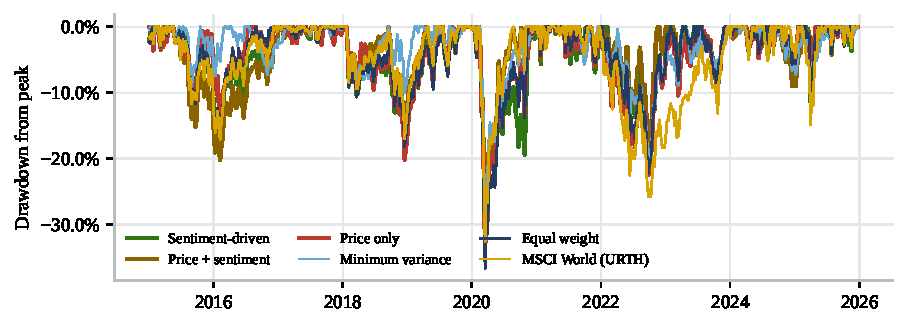
\includegraphics[width=\textwidth]{drawdown}
\caption{Drawdown from the previous peak after costs, 2015--2025.}\label{fig:drawdown}\end{figure}
\begin{figure}[H]\centering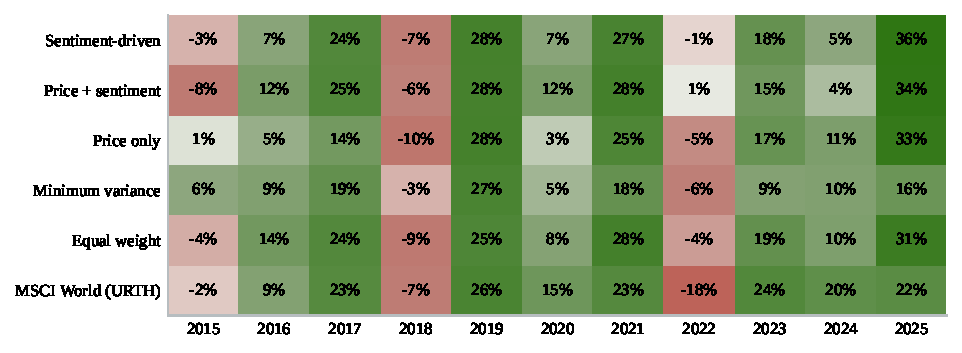
\includegraphics[width=\textwidth]{annual}
\caption{Net annual returns by strategy and year.}\label{fig:annual}\end{figure}

\section{Reproduction}\label{app:code}
{\sloppy All results, tables and figures are produced from the stored data by \texttt{project.py} in four stages: \texttt{validate-price} and \texttt{validate-sentiment} (2012--2014 only), \texttt{freeze}, which stores a SHA-256 fingerprint of the code, settings and validation choices, and \texttt{test}, which refuses to run if anything changed after freezing and runs only once. Package versions and input file hashes are recorded in \texttt{results/test\_run.json}.\par}

\end{document}
